\chapter{Medidas para Masking-tolerancia a fallas}
\label{cap:maskingMeasure}

\myworries{REVISAR PRUEBAS} \\
Introducimos una noción de distancia de tolerancia a fallas entre sistemas de transición etiquetados. Intuitivamente, esta noción de distancia mide el grado de tolerancia a fallas exhibido por un sistema candidato.
En la práctica, hay diferentes tipos de tolerancia a fallas, aquí nos restringimos al análisis de masking-tolerancia a fallas ya que suele ser una característica muy deseada para sistemas críticos.
En términos generales, un sistema es masking-tolerante a fallas cuando es capaz de enmascarar las fallas completamente, sin permitir que estas fallas tengan consecuencias observables para los usuarios.
Capturamos la masking-tolerancia a fallas mediante una relación de simulación, acompañada por una caracterización correspondiente en términos de juegos.
Enriquecemos además estos juegos con objetivos cuantitativos para así definir la noción de distancia de masking-tolerancia a fallas.
Además, investigamos las propiedades básicas de esta noción de distancia de masking y probamos que es una semi-métrica dirigida.
Demostramos que, en el caso de sistemas deterministas, computar la distancia de masking se puede lograr utilizando un algoritmo de camino más corto.
Por otro lado, para sistemas no deterministas este cómputo se aborda por medio de algoritmos de punto fijo.
Estos algoritmos fueron implementados en una herramienta que computa de manera automática la distancia de masking entre un sistema nominal y una versión del mismo que agrega fallas (y mecanismos de tolerancia). Hemos evaluado su desempeño y efectividad sobre varios casos de estudio de diferentes complejidades.



\section{Introducción} \label{sec:intro_mask}

La tolerancia a fallas es una característica importante del software crítico, y puede ser definida como la capacidad de un sistema para lidiar con eventos inesperados, que pueden ser causados por bugs de programación, interacciones con un ambiente poco cooperativo, mal funcionamiento de hardware, etcétera.
Se pueden encontrar ejemplos de sistemas tolerantes a fallas en casi cualquier parte: protocolos de comunicación, circuitos de hardware, sistemas de aviación, criptomonedas, etcétera.
Por lo tanto, el incremento en la relevancia del software crítico en la vida cotidiana ha llevado a que se renueve el interés en la verificación automática de propiedades de tolerancia a fallas. Sin embargo, una de las dificultades principales a la hora de razonar sobre estos tipos de propiedades se da en su naturaleza cuantitativa, lo cual es cierto incluso en sistemas no probabilistas.
Un ejemplo simple se da con la introducción de redundancia en sistemas críticos. Esta es, sin lugar a dudas, una de las técnicas más utilizadas en tolerancia a fallas.
En la práctica, es común añadir más redundancia en un sistema para incrementar su confiabilidad. Medir este incremento de confiabilidad es un problema central a la hora de evaluar software tolerante a fallas. Por otro lado, no hay un método \emph{de-facto} para caracterizar formalmente propiedades tolerantes a fallas, y por ello se suelen codificar utilizando mecanismos \emph{ad-hoc} como parte del diseño general.

Usualmente el flujo del diseño y verificación de sistemas tolerantes a fallas consiste en definir un modelo nominal (es decir, el programa ``sin fallas'' o ``ideal'') y luego extenderlo con comportamientos defectuosos que se desvían del comportamiento normal descrito por el modelo nominal.
Este modelo extendido representa la manera en la que el sistema opera bajo la ocurrencia de fallas.
Hay diferentes maneras de extender el modelo nominal, el enfoque típico involucra la \emph{inyección de fallas}  \cite{HsuehTI97,IyerNGK10}, es decir, la introducción automática de fallas en el modelo. Una propiedad importante que cualquier modelo extendido debería satisfacer es la preservación del comportamiento normal ante la ausencia de fallas.
En \cite{DemasiCMA17} se propone un enfoque formal alternativo para tratar con el análisis de la tolerancia a fallas. Este enfoque permite un análisis totalmente automático y distingue apropiadamente comportamientos defectuosos y normales. Además, este \textit{framework} es sensible a la inyección de fallas. En ese trabajo se definen tres nociones de relaciones de simulación para caracterizar diferentes tipos de tolerancia a fallas:
tolerancia \emph{enmascarante}, \emph{no enmascarante}, y \emph{seguro ante fallos}, originalmente definidas en \cite{Gartner99}. 

Por otro lado, en los últimos años, se ha logrado un progreso significativo en pos de definir métricas, o nociones de distancias, apropiadas para diversos tipos de modelos cuantitativos, incluyendo sistemas de tiempo real \cite{HenzingerMP05}, modelos probabilistas \cite{DesharnaisGJP04}, y métricas para sistemas lineales y ramificados \cite{CernyHR12,AlfaroFS09,Henzinger13,LarsenFT11,ThraneFL10}. 
Algunos autores han resaltado que estas métricas pueden ser útiles para razonar sobre la robustez de un sistema, un concepto relacionado con la tolerancia a fallas. Particularmente, en \cite{CernyHR12}, la noción tradicional de relación de simulación se generaliza, y se introducen tres distancias de simulación entre sistemas, concretamente \emph{correctitud}, \emph{cobertura}, y \emph{robustez}.
A estas distancias se las define utilizando juegos cuantitativos con objetivos \emph{discounted-sum} y \emph{mean-payoff}.

En este capítulo introducimos una noción de distancia de tolerancia a fallas entre sistemas de transición etiquetados. Intuitivamente, esta distancia mide el grado de tolerancia a fallas exhibido por un sistema candidato. Como fue mencionado anteriormente, existen varios niveles de tolerancia a fallas, aquí nos restringimos al análisis de \emph{tolerancia a fallas enmascarante} ya que usualmente se la considera como el tipo de tolerancia mas beneficioso y por lo tanto es una propiedad altamente deseable en cualquier sistema critico.
A grandes rasgos, un sistema es tolerante a fallas de forma enmascarante cuando es capaz de enmascarar completamente las fallas, no permitiendo que las mismas tengan consecuencias observables para los usuarios. Formalmente, el sistema debe preservar tanto las propiedades de \textit{safety} como las de \textit{liveness} del modelo nominal \cite{Gartner99}. A diferencia de la distancia de robustez definida en \cite{CernyHR12}, la cual mide cuantos errores inesperados son tolerados por una implementación, aquí consideramos una colección especifica de fallas dadas en la implementación y medimos cuantas fallas son toleradas por la implementación de tal manera que puedan ser enmascaradas por los estados del sistema.
También requerimos que el comportamiento normal de la especificación se preserve en la implementación cuando no hay fallas.
Por lo tanto, distinguimos efectivamente entre el modelo nominal, su versión tolerante a fallas,  y el conjunto de fallas para el sistema en cuestión.

Para poder medir el grado de tolerancia a fallas enmascarante de un sistema dado, empezamos caracterizando la tolerancia a fallas enmascarante por medio de relaciones de simulación entre dos sistemas, como se define en \cite{DemasiCMA17}. El primero cumple el rol de especificación del comportamiento deseado (es decir, el modelo nominal) y el segundo cumple el rol de una implementación tolerante a fallas (es decir, el modelo extendido con fallas y mecanismos de tolerancia).
La existencia de una relación de enmascaramiento implica que la implementación enmascara todas las fallas consideradas. Luego, introducimos una caracterización de la simulación de enmascaramiento en términos de juegos y enriquecemos los mismos con objetivos cuantitativos para definir así la noción de \emph{distancia de tolerancia a fallas enmascarante} o \emph{distancia de enmascaramiento}, donde los valores posibles del juego pertenecen al intervalo  $[0,1]$. 
Formalmente, dado un sistema nominal $N$ y su implementación $I$ y sea $\DeltaMask$ nuestra función de distancia, tenemos que $\DeltaMask(N,I)=0$ si la $I$ es tolerante a fallas con enmascaramiento respecto de $N$. Además, mientras mayor el valor, más lejos está la implementación de la especificación en términos de la distancia de tolerancia a fallas enmascarante. De esta forma, una distancia mayor decrementa notablemente el grado de tolerancia a fallas. A su vez, $\DeltaMask(N,I)=1$ cuando el modelo nominal $N$ y $I \backslash F$ no son bisimilares, donde $I\backslash F$ se comporta como la implementación $I$ cuando todas las acciones en $F$ están deshabilitadas ($\backslash$ es el operador de restricción de Milner).
Entonces, para un modelo nominal $N$ y dos implementaciones tolerantes a fallas diferentes $I_1$ y $I_2$, nuestra distancia asegura que  $\DeltaMask(N,I_1)<\DeltaMask(N,I_2)$ cuando $I_1$ tolera mas fallas que $I_2$.
También proporcionamos una versión débil de la simulación de enmascaramiento, la cual hace posible tratar con sistemas más complejos compuestos por varios componentes que interactúan entre si. Probamos que la distancia de enmascaramiento es una semi-métrica dirigida, es decir, que satisface dos propiedades básicas de cualquier distancia: reflexividad y la desigualdad triangular.

Finalmente, hemos implementado nuestra técnica en una herramienta que toma como argumentos un modelo nominal y su implementación tolerante a fallas, y computa automáticamente la distancia de enmascaramiento entre estos.
Hemos utilizado esta herramienta para medir tolerancia a fallas enmascarante en múltiples instancias de varios casos de estudio: una celda de memoria redundante \cite{DemasiCMA17}, una variante del problema de los filósofos comensales \cite{Dijkstra71}, el protocolo de comunicación BRP (\emph{Bounded Retransmission Protocol}) \cite{GrooteP96}, redundancia N-Modular \cite{ShoomanBook}, el problema de los generales bizantinos \cite{LamportSP82} y un subproblema del protocolo de consenso Raft \cite{OngaroO14} para lograr una replicación consistente de datos.
Todos los casos de estudio mencionados son ejemplos típicos de sistemas tolerantes a fallas. Un punto interesante sobre nuestra implementación es que, para sistemas deterministas, la distancia de enmascaramiento entre dos sistemas puede ser computada recurriendo a un algoritmo de camino más corto. Mientras que en el caso de sistemas no deterministas, se aplica un algoritmo de punto fijo basado en la búsqueda primero a lo ancho (\emph{breadth first search}), lo cual es menos eficiente, sin embargo en ambos casos el algoritmo es polinomial. Los detalles de la herramienta quedan delegados al Capítulo~\ref{cap:tool}.

El capítulo está estructurado de la siguiente manera. La sección \ref{sec:masking_dist_mask} presenta la definición de simulación de enmascaramiento (fuerte y débil) y la caracterización de juegos correspondiente.
En la Sección \ref{sec:QuantMask_mask} presentamos la definición formal de distancia de enmascaramiento que se construye a partir de juegos de simulación cuantitativos, presentamos también los algoritmos para computarla, y también probamos sus propiedades elementales.
Se describe en la Sección \ref{sec:experimental_eval_mask} la evaluación experimental sobre varios casos de estudio conocidos. 
Finalmente en la Sección \ref{sec:related_work_mask} discutimos el trabajo relacionado. 
\section{Simulación de Enmascaramiento (o \textit{Masking})}
\label{sec:masking_dist_mask}
%Empezamos definiendo la simulación de masking. En \cite{DemasiCMA17}, se definió una simulación basada en estados para la masking-tolerancia a fallas, aquí reformulamos esta definición usando simulación basada en transiciones. Primero, vamos a introducir algunos conceptos que son necesarios para definir masking-tolerancia a fallas. Para todo vocabulario $\Sigma$, y todo conjunto de etiquetas $\Faults = \{F_0, \dots, F_n\}$ no pertenecientes a $\Sigma$, consideramos $\SigmaF = \Sigma \cup \Faults$, donde $\Faults \cap \Sigma = \emptyset$. 
La simulación de enmascaramiento provee una forma de verificar si una implementación tolerante a fallas es correcta al comprobar que un modelo que sirve de implementación (el cuál incluye fallas y mecanismos de tolerancia a fallas) se comporta como el modelo nominal (es decir, la especificación del sistema asumiendo que no hay fallas) siguiendo reglas del estilo de una bisimulación.
En \cite{DemasiCMA17}, se definió una simulación basada en estados para la tolerancia a fallas enmascarante, aquí reformulamos esta definición usando simulación basada en transiciones. 

Para todo vocabulario $\Sigma$, y todo conjunto de etiquetas $\Faults = \{F_0, \dots, F_n\}$ con $\Faults \cap \Sigma = \emptyset$, consideramos $\SigmaF = \Sigma \cup \Faults$. 
Intuitivamente, los elementos de $\Faults$ indican la ocurrencia de una falla en una implementación defectuosa. Además, a veces será útil considerar el conjunto $\Sigma^i = \{ e^i \mid e \in \Sigma\}$, que contiene los elementos de $\Sigma$ indexados con el superíndice $i$.

%, $\Sigma^i = \{\sigma^i \mid \sigma \in \Sigma\}$.

\subsection{Simulación de Enmascaramiento Fuerte}
\begin{definition} \label{def:masking_rel}
  Sean $A =\langle S, \Sigma, \rightarrow, s_0\rangle$ y $A' =\langle S', \SigmaF, \rightarrow', s_0' \rangle$ dos sistemas de transición etiquetados.
  $A'$ es \emph{fuertemente tolerante a fallas enmascarante} con respecto a $A$ si existe una relación 
$\M \subseteq S \times S'$ entre $A$ y $A'$ tal que:

\begin{enumerate}[(A)]
  \item $s_0 \M s'_0$, y
  \item para todo $s \in S, s' \in S'$ con $s \M s'$ y todo $e \in \Sigma$ vale lo siguiente:

  \begin{enumerate}[(1)]
    \item 
    si $s \xrightarrow{e} t$ entonces
    $\exists\; t' \in S': s' \xrightarrowprime{e} t'  \wedge t \M t'$;

      \item si $s' \xrightarrowprime{e} t'$ entonces
      $\exists \; t \in S: s \xrightarrow{e} t \wedge t \M t'$;

      \item si $s' \xrightarrowprime{F} t' $ para algún $F \in \Faults$ entonces
      $s \M t'$.
      
  \end{enumerate}
\end{enumerate}

Si tal relación existe, decimos que $A'$ es una \emph{implementación fuertemente tolerante a fallas enmascarante} de $A$, denotado como $A \Masking A'$. 
\end{definition}

Observemos que la definición es la estándar de bisimulación fuerte a excepción de que las etiquetas de fallas son tratadas de forma diferente ya que solo aparecen en el modelo de la implementación.  En este sentido, una falla producida por la implementación $A'$ es enmascarada apropiadamente si permanece desapercibida por el modelo nominal $A$ (ver regla (B.3)).
%
Más específicamente, la condición (A) establece que $A$ y $A'$ se relacionan en sus estados iniciales, y las condiciones (B.1) y (B.2) son las propiedades de transferencia típicas de bisimulaciones limitadas a el comportamiento nominal (es decir todas las transiciones que no están etiquetadas como fallas).
%
Sin embargo, la condición (B.3) establece que siempre que una falla se produzca en el modelo de la implementación $A'$, el modelo nominal $A$ solo puede imitar la acción quedándose en el mismo estado (es decir, haciendo nada).
%Intuitivamente, la definición establece que, partiendo de $s'$, las fallas pueden ser enmascaradas de tal forma que el comportamiento exhibido es el mismo que el observado al partir de $s$ ejecutando transiciones sin fallas. 
%En otras palabras, una relación de masking asegura que cualquier comportamiento defectuoso en la implementación puede ser simulado por la especificación. Mas específicamente, note que las condiciones (A), (B.1) y (B.2) implican que tenemos una bisimulación cuando $A$ y $A'$ no exhiben comportamientos defectuosos.
%Particularmente, la condición (B.1) dice que la ejecución normal de $A$ puede ser simulada por una ejecución de $A'$. Por otro lado, la condición (B.2) dice que la implementación no agrega más comportamientos normales (no defectuosos). Por ultimo, la condición (B.3) establece que toda transición defectuosa ($F$) que salga de $s'$ debe ser emparejada por un movimiento de $s$ a si mismo (es decir la especificación no hace nada).

\subsection{Simulación de Enmascaramiento Débil}

Para analizar sistemas menos triviales se necesita una relación de simulación de enmascaramiento débil. La idea principal es que una simulación de enmascaramiento débil se abstrae del comportamiento interno, el cual es modelado por una acción especial $\tau$. Observemos que las transiciones internas son comunes en tolerancia a fallas: las acciones ejecutadas como parte de un mecanismo tolerante a fallas en un componente usualmente no son observables para el resto del sistema.

Sea $A =\langle S, \Sigma \cup \{\tau\} \cup \Faults,  \rightarrow, s_0\rangle$ un sistema de transición etiquetado. Primero, consideremos la relación binaria ${\Rightarrow} \subseteq S \times S$ definida como la clausura reflexo-transitiva de $\xrightarrow{\tau}$, es decir, ${\Rightarrow} = {\xrightarrow{\tau}^*}$.  En otras palabras, decimos que $s \Rightarrow s'$ si hay un camino finito:  $s_0 \xrightarrow{\tau} s_2 \xrightarrow{\tau} \dots \xrightarrow{\tau} s_n$ tal que $s = s_0$, $s' = s_n$ y $n \geq 0$.
 %$\Sigma$ contains a distinguished \textit{silent} action $\tau$.
$\Rightarrow$ se puede extender a una relación etiquetada ${\Rightarrow} \subseteq S\times (\Sigma \cup \{\tau\} \cup \Faults) \times S$ de la siguiente manera: para todo $s,s'\in S$ y $e\in {\Sigma \cup \{\tau\} \cup \Faults}$,
 %for all $e \in \Sigma \cup \{\tau\}$ in such a way that $\Rightarrow$ (also denoted as $E_W$)  
 %is the relation $E$ preceded and followed by a arbitrary number of $\tau$ transitions. Formally:\\
 %
 \[
s \xRightarrow{e} s' \text{ \ ssi \ }
        \begin{cases}
            \exists t,t'\in S \colon s \Rightarrow t \xrightarrow{e} t' \Rightarrow s' & 
             \text{si } e \in \Sigma,  \\ 
            s \Rightarrow s' & \text{si } e = \tau,  \\
            s \xrightarrow{e} s' & \text{si } e \in \Faults.\\
        \end{cases}
 \]
 %
%The symbol $\circ$ stands for composition of binary relations.
 
 %

%Las \textit{relaciones de transición débiles} ${\Rightarrow} \subseteq S
%\times (\Sigma \cup \{\tau\} \cup \Faults) \times S$ consideran el paso \emph{silencioso} $\tau$ que se define como sigue: 

%\[
%\xRightarrow{e} = 
%       \begin{cases}
%            \xrightarrowstar{\tau} \circ \xrightarrow{e} \circ \xrightarrowstar{\tau} & 
%            \text{si } e \in \Sigma,  \\ 
%            \xrightarrowstar{e} & \text{si } e = \tau,  \\
%            \xrightarrow{e} & \text{si } e \in \Faults.\\
%       \end{cases}
%\]
%
%El símbolo $\circ$ representa la composición de relaciones binarias y $\xrightarrowstar{\tau}$ es la clausura reflexo-transitiva de la relación binaria $\xrightarrow{\tau}$. 

Intuitivamente, si $e \notin \{\tau\}\cup\Faults$, entonces $s\xRightarrow{e}s'$ significa que existe una secuencia de cero o mas transiciones $\tau$ empezando en $s$, seguido de una transición etiquetada por $e$, seguida luego por cero o mas transiciones $\tau$ eventualmente llegando a  $s'$.
$s \xRightarrow{\tau} s'$ establece que $s$ puede moverse a $s'$ por medio de cero o mas transiciones $\tau$.
%
En particular, $s \xRightarrow{\tau} s$ para todo $s$.
%
Para el caso en que $e\in\Faults$,
$s\xRightarrow{e}s'$ es equivalente a $s\xrightarrow{e}s'$ y por lo tanto no se permite ningún paso $\tau$ antes o después de la transición $e$.

\begin{definition} \label{def:weak_mask}
  Sean $A =\langle S, \Sigma, \rightarrow, \InitState \rangle$ y $A' =\langle S',
  \SigmaF, \rightarrow', \InitStatePrime \rangle$ dos sistemas de transición etiquetados con $\Sigma$
  conteniendo $\tau$ posiblemente.  $A'$ es \emph{débilmente tolerante a fallas enmascarante}
  con respecto a $A$ si existe una relación $\M \subseteq S
  \times S'$ entre $A$ y $A'$ tal que:

\begin{enumerate}[(A)]
  \item $\InitState \M \InitStatePrime$
  \item para todo $s \in S, s' \in S'$ con $s \M s'$ y todo $e \in \Sigma \cup \{\tau\}$ vale lo siguiente:

  \begin{enumerate}[(1)]
    \item si $s \xrightarrow{e} t$ entonces 
    $\exists\; t' \in S': s' \xRightarrowprime{e} t' 
    \wedge t \M t'$;

      \item si $s' \xrightarrowprime{e} t'$ entonces  
      $\exists \; t \in S: s \xRightarrow{e} t  
      \wedge t \M t'$;

      \item si $s' \xrightarrowprime{F} t'$ para algún $F \in \Faults$ entonces 
      $s \M t'$.
  \end{enumerate}
\end{enumerate}

%
Si tal relación existe, decimos que $A'$ es una \emph{implementación débilmente tolerante a fallas enmascarante} de
$A$, denotado por $A \WeakMasking A'$.
\end{definition}

El siguiente teorema conecta la simulación de enmascaramiento fuerte con la débil. El teorema establece que la simulación de enmascaramiento débil se vuelve una simulación de enmascaramiento fuerte cuando la transición $\xrightarrow{}$ es reemplazada por $\xRightarrow{}$ en la estructura original.

\begin{theorem} \label{thm:weak_thm}
  Sean
$A =\langle S, \Sigma, \rightarrow, \InitState \rangle$ y $A' =\langle S', \SigmaF, \rightarrow', \InitStatePrime \rangle$. 
$\M \subseteq S \times S'$ entre $A$ y $A'$ es una simulación de enmascaramiento débil si y solo si:

\begin{enumerate}[(A)]
  \item $\InitState \M \InitStatePrime$, y
  \item para todo $s \in S, s' \in S'$ con $s \M s'$ y todo $e \in \Sigma \cup \{\tau\}$ vale lo siguiente:

  \begin{enumerate}[(1)]
    \item si $s \xRightarrow{e} t$ entonces $\exists\; t' \in S': s' \xRightarrowprime{\text{e}} t' 
    \wedge t \M t'$;

      \item si $s' \xRightarrowprime{e} t'$ entonces 
      $\exists \; t \in S: s \xRightarrow{e} t \
      \wedge t \M t')$;

      \item si $s' \xRightarrowprime{F} t'$ para algún $F \in \Faults$ entonces 
      $s \M t'$
  \end{enumerate}
\end{enumerate}

\end{theorem}

\noindent
\begin{proof}
Primero observemos que las condiciones (A), (B.1), (B.2) y (B.3) de este teorema implican directamente a las condiciones (A), (B.1), (B.2) y (B.3) de la Definición~\ref{def:weak_mask}, respectivamente. Por lo tanto, la parte ``si'' de la prueba es directa. Para la parte ``solo si'', la condición (A) es la misma tanto en el teorema como en la definición.
Para la condición (B), tomamos $s \M s'$ y procedemos de la siguiente forma.

Para (B.1), asumamos que $s \xRightarrow{e} t$ para $e \in \Sigma \cup \{\tau\}$ y $t \in S$.
Procedemos por casos.

Si $e = \tau$, entonces, por definición de $\xRightarrow{\tau}$, existen $s_0,s_1,\ldots,s_n$ con $n\geq0$ tal que $s=s_0\xrightarrow{\tau}s_1\xrightarrow{\tau}{\cdots}\xrightarrow{\tau}s_n=t$.
%
Por la propiedad (B.1) de la Definición~\ref{def:weak_mask}, existen $s'_0,s'_1,\ldots,s'_n$ tal que $s'=s'_0\xRightarrowprime{\tau}s'_1\xRightarrowprime{\tau}{\cdots}\xRightarrowprime{\tau}s'_n$ y $s_i \M s'_i$ para $0<i\leq n$. Por lo tanto $s' \xRightarrowprime{\tau} t'$ y $t \M t'$ al tomar $t'=s'_n$.

Si $e \in \Sigma$, por definición de $\xRightarrow{\tau}$, existen $\hat{s}$ y $\hat{t}$ tal que $s\xRightarrow{\tau}\hat{s}\xrightarrow{e}\hat{t}\xRightarrow{\tau}t$.
Debido al caso previo para $\xRightarrow{\tau}$, y (B.1) de la Definición~\ref{def:weak_mask} para $\xRightarrow{e}$, existen $s'$, $\hat{s}'$, $\hat{t}'$ y $t'$ tal que $s'\xRightarrowprime{\tau}\hat{s}'\xRightarrowprime{e}\hat{t}'\xRightarrowprime{\tau}t'$ con $\hat{s} \M \hat{s}'$, $\hat{t} \M \hat{t}'$ y $t \M t'$.
Por lo tanto, $s'\xRightarrowprime{e}t'$ y $t \M t'$.

La condición (B.2) se deduce de forma similar.

Para (B.3), supongamos $s' \xRightarrowprime{F} t'$ para algún $t' \in S'$.  Entonces, por definición de ${\xRightarrowprime{F}}$, $s' \xrightarrowprime{F} t'$.  Utilizando la propiedad (B.3) de la Definición~\ref{def:weak_mask} se deduce que $s \M t'$, lo cual concluye la prueba.
%Primero observemos que las condiciones (A), (B.1), (B.2) y (B.3) en este teorema implican las condiciones (A), (B.1), (B.2) y (B.3)
% de la Definición~\ref{def:weak_mask}, entonces la parte ``si'' es directa. Para la otra dirección, la condición (A) es la misma en el teorema y en la definición.
% Supongamos ahora que la condición (B.1) de la Definición~\ref{def:weak_mask} vale, es decir,
% $s \xRightarrow{e} t$ para $e \in \Sigma \cup \{\tau\}$ y $t \in S$. 
%Si $e \in \Sigma$, entonces, por definición de$\Rightarrow$, tenemos que existen $w$ y $v$ tal que $s \xrightarrowstar{\tau} w$, $w \xrightarrow{e} v$
% y $v \xrightarrowstar{\tau} t$. Por lo tanto, por definición de $\Rightarrow$ y por la condición (B.2) de la Definición \ref{def:weak_mask} 
% tenemos que existen estados $s',t',w',v' \in S'$
% tales que $s' \xRightarrow{\tau} w'$, $w' \xRightarrow{e} v'$, y $v' \xRightarrow{\tau} t'$ y, 
% además, $w \M w'$, $v \M v'$, y $t \M t'$ lo cual implica que$s' \xRightarrow{e} t'$. 
% La prueba para la condición (B.2) es similar.
% 	Supongamos ahora que $s \M s'$ y $s' \xRightarrow{F} t'$, para algún $t' \in S'$. Entonces, por Definición de 
%$\Rightarrow$, tenemos que $s' \xrightarrow{F} t'$ y por Definición~\ref{def:weak_mask}
% tenemos $s \M t'$ . Esto concluye la prueba.
 \qedhere 
 \end{proof} 
 
Una forma natural de verificar bisimilitud débil es por medio de \emph{saturar}
el sistema de transición  \cite{FernandezM91,Milner89} y luego verificar bisimilitud fuerte sobre el sistema de transición saturado.
Similarmente, el Teorema~\ref{thm:weak_thm} nos permite computar simulación de enmascaramiento débil sobre $A =\langle S, \Sigma, \rightarrow, \InitState \rangle$ y $A' =\langle S', \SigmaF, \rightarrow', \InitStatePrime \rangle$ al reducir este problema al de computar simulación de enmascaramiento fuerte sobre las versiones saturadas $\textrm{sat}(A) =\langle S, \Sigma, \Rightarrow, \InitState \rangle$ y $\textrm{sat}(A') =\langle S', \SigmaF, \Rightarrow', \InitStatePrime \rangle$. 

En lo que resta del capítulo utilizaremos el Teorema~\ref{thm:weak_thm} para demostrar propiedades sobre enmascaramiento débil. Vale la pena destacar que la mayoría de las propiedades de enmascaramiento fuerte pueden ser también demostradas para enmascaramiento débil aplicando el Teorema~\ref{thm:weak_thm}.
	
\begin{example}
Consideremos el siguiente ejemplo, consideramos una celda de memoria que almacena un bit de información y soporta operaciones de lectura y escritura, presentado en forma basada en estados en \cite{DemasiCMA17}. Un estado en este sistema mantiene el valor corriente de la celda de memoria ($m=i$, para $i=0,1$), escribir le permite a uno cambiar este valor, y leer retorna el valor almacenado.  
Obviamente, en este sistema el resultado de una lectura va a depender del valor almacenado en la celda. 
Por lo tanto, una propiedad que uno podría asociar a este modelo es que el valor leído de la celda coincida con el de la ultima escritura que se haya ejecutado en el sistema.
    
Una falla que potencialmente se puede dar en este escenario ocurre cuando la celda inesperadamente pierde su carga, y su valor almacenado cambia (e.g., cambia de $1$ a $0$ debido a perdida de carga). Una técnica típica para lidiar con esta situación es \emph{redundancia}: usar tres bits de memoria en lugar de solo uno. Las operaciones de escritura se realizan simultáneamente sobre los tres bits. La lectura, por otro lado, retorna el valor que se repite en la mayoría de bits, esto se conoce como \emph{votación}. 

Adoptamos el siguiente enfoque para modelar este sistema. Las etiquetas $\text{w}_0, \text{w}_1, \text{r}_0,$ y $\text{r}_1$
representan las operaciones de escritura y lectura. Específicamente, $\text{w}_0$ (resp. $\text{w}_1$): escribe el valor cero (resp. uno) en la celda de memoria. $\text{r}_0$ (resp. $\text{r}_1$): lee el valor cero (resp. uno) almacenado en la celda de memoria.
La Figura~\ref{figure:exam_1_mem_cell} muestra tres sistemas de transición de estados. El primero de izquierda a derecha representa el sistema nominal para este ejemplo (denotado como $A$).
Tanto el segundo como el tercer sistema de transición son implementaciones tolerantes a fallas de $A$, denotados como $A'$ y $A''$ respectivamente. Observemos que $A'$ contiene una falla, mientras que $A''$ considera dos fallas. Ambas implementaciones usan redundancia triple; intuitivamente, el estado $\text{t}_0$ contiene tres bits con valor cero y $\text{t}_1$ contiene tres bits con valor uno.
Además, el estado $\text{t}_2$ se alcanza cuando uno de los bits cambió de valor (001, 010 o 100)
En  $A''$, el estado $\text{t}_3$ se alcanza después de que cambia un segundo bit (011, 101 o 110) empezando del estado $\text{t}_0$.
%\begin{figure}[h] 
%\begin{center}
%    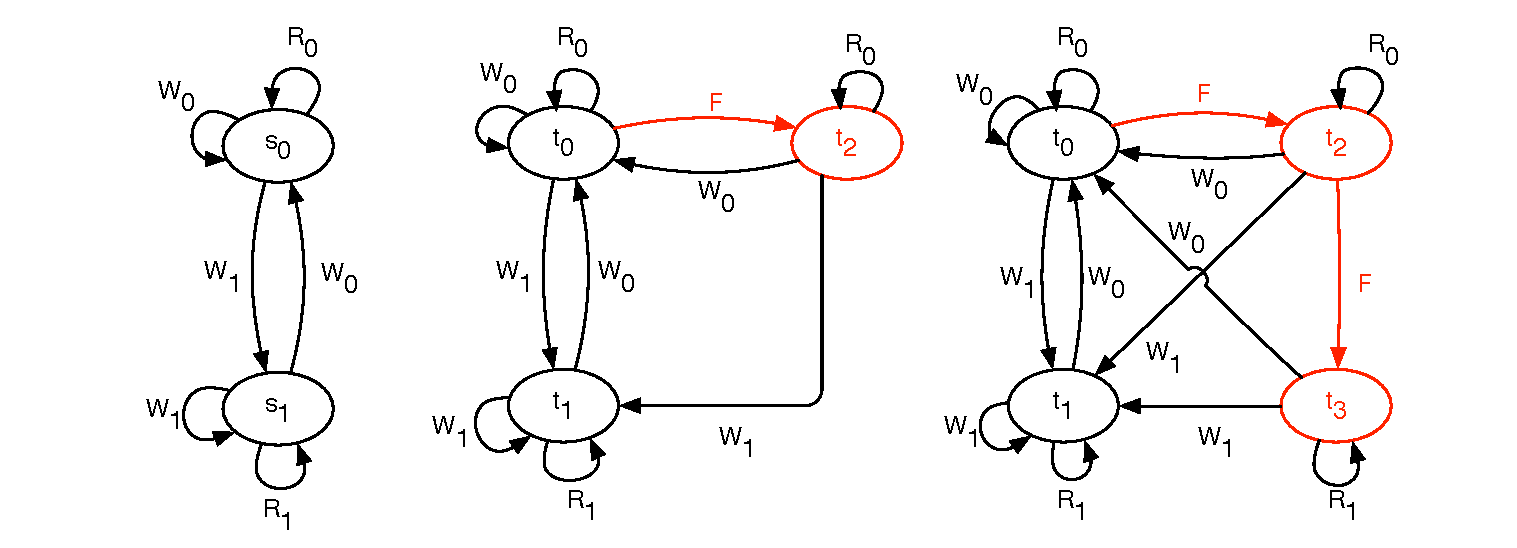
\includegraphics[scale=0.45]{Figs/example_1_cell_mem-eps-converted-to.pdf} 
   % \vspace{-1cm}
%    \caption{Modelo nominal y dos modelos con fallas de una celda de memoria.}
    %\vspace{-0.8cm}
%    \label{figure:exam_1_mem_cell}
%\end{center}
%\end{figure}
\begin{figure}[ht] 
\begin{center}
  % \includegraphics[scale=0.45]{example_1_cell_mem.eps} 
  % \vspace{-1cm}
  \begin{subfigure}{.26\textwidth}\centering
  \scalebox{1.1}{
  \begin{tikzpicture}[on grid,auto,align at top]
    \node[state] (n0)                   {$s_0$};
    \node[state] (n1) [below=2.3 of n0] {$s_1$};

    \path[-Latex]
    (n0) edge[bend right=15] node[swap] {$w_1$} (n1)
    (n0) edge[loop,out=60,in=120,looseness=5] node[above] {$w_0$} (n0)
    (n0) edge[loop,out=150,in=210,looseness=5] node[left] {$r_0$} (n0)
    (n1) edge[bend right=15] node[swap] {$w_0$} (n0)
    (n1) edge[loop,out=-60,in=-120,looseness=5] node[below] {$r_1$} (n1)
    (n1) edge[loop,out=150,in=210,looseness=5] node[left] {$w_1$} (n1)
    ;
  \end{tikzpicture}
  }
  \caption{Modelo nominal $A$}\label{figure:exam_1_mem_cell:nominal}
  \end{subfigure}
  %\hfill
  \begin{subfigure}{.32\textwidth}\centering
  \scalebox{1.1}{
  \begin{tikzpicture}[on grid,auto,align at top]
    \node[state] (n0)                   {$t_0$};
    \node[state] (n1) [below=2.3 of n0] {$t_1$};
    \node[state,red,fill=white,text=red] (n2) [right=2.3 of n0] {$t_2$};

    \path[-Latex]
    (n0) edge[red,bend left=15]  node {$F$}   (n2)
    (n0) edge[bend right=15] node[swap] {$w_1$} (n1)
    (n0) edge[loop,out=60,in=120,looseness=5] node[above] {$w_0$} (n0)
    (n0) edge[loop,out=150,in=210,looseness=5] node[left] {$r_0$} (n0)
    (n1) edge[bend right=15] node[swap] {$w_0$} (n0)
    (n1) edge[loop,out=-60,in=-120,looseness=5] node[below] {$r_1$} (n1)
    (n1) edge[loop,out=150,in=210,looseness=5] node[left] {$w_1$} (n1)
    (n2) edge[loop,out=60,in=120,looseness=5] node[above] {$r_0$} (n2)
    (n2) edge[bend left=15] node {$w_0$} (n0)
    (n2) edge[bend left=45] node {$w_1$} (n1)
    ;
  \end{tikzpicture}
  }
  \caption{Modelo con una falla $A'$}\label{figure:exam_1_mem_cell:onefault}
  \end{subfigure}
  %\hfill
  \begin{subfigure}{.32\textwidth}\centering
  \scalebox{1.1}{
  \begin{tikzpicture}[on grid,auto,align at top]
    \node[state] (n0)                   {$t_0$};
    \node[state] (n1) [below=2.3 of n0] {$t_1$};
    \node[state,red,fill=white,text=red] (n2) [right=2.3 of n0] {$t_2$};
    \node[state,red,fill=white,text=red] (n3) [below=2.3 of n2] {$t_3$};

    \path[-Latex]
    (n0) edge[red,bend left=15]  node {$F$}   (n2)
    (n0) edge[bend right=15] node[swap] {$w_1$} (n1)
    (n0) edge[loop,out=60,in=120,looseness=5] node[above] {$w_0$} (n0)
    (n0) edge[loop,out=150,in=210,looseness=5] node[left] {$r_0$} (n0)
    (n1) edge[bend right=15] node[swap] {$w_0$} (n0)
    (n1) edge[loop,out=-60,in=-120,looseness=5] node[below] {$r_1$} (n1)
    (n1) edge[loop,out=150,in=210,looseness=5] node[left] {$w_1$} (n1)
    (n2) edge[red]  node {$F$}   (n3)
    (n2) edge[loop,out=60,in=120,looseness=5] node[above] {$r_0$} (n2)
    (n2) edge[bend left=15] node {$w_0$} (n0)
    (n2) edge node[pos=0.25,inner sep=1pt] {$w_1$} (n1)
    (n3) edge node {$w_1$} (n1)
    (n3) edge[loop,out=-60,in=-120,looseness=5] node[below] {$r_1$} (n3)
    (n3) edge node[swap,pos=0.25,inner sep=1pt] {$w_0$} (n0)
    ;
  \end{tikzpicture}
  }
  \caption{Modelo con dos fallas $A''$}\label{figure:exam_1_mem_cell:twofaults}
  \end{subfigure}

  \caption{LTS para la celda de memoria.}
  %\vspace{-0.8cm}
  \label{figure:exam_1_mem_cell}
\end{center}
\end{figure}
\sloppy No es difícil ver que existe una relación de tolerancia a fallas enmascarante entre $A$ y $A'$, teniendo como testigo la relación $\M = \{(\text{s}_0, \text{t}_0), (\text{s}_1, \text{t}_1), (\text{s}_0, \text{t}_2)\}$. Es sencillo verificar que $\M$ satisface las condiciones de la Definición~\ref{def:masking_rel}.

Por otro lado, no existe una relación de enmascaramiento entre $A$ y $A''$ ya que el estado $\text{t}_3$ necesita estar relacionado con el estado $\text{s}_0$ en cualquier relación de enmascaramiento entre estos modelos. Este estado solo puede ser alcanzado con la ejecución de fallas, las cuales son necesariamente enmascaradas por transiciones ficticias. Sin embargo, observemos que, en el estado $\text{t}_3$, se puede leer el valor $1$ (la transición $\text{t}_3 \xrightarrow{\text{r}_1} \text{t}_3$) mientras que, en el estado $\text{s}_0$, solo se puede leer el valor $0$ (la transición $\text{s}_0 \xrightarrow{\text{r}_0} \text{s}_0$).
\end{example}
 
\subsection{Juego de Simulación de Enmascaramiento} \label{subsec:mask_sim_game}
Aquí procedemos a definir un juego de simulación de enmascaramiento para dos sistemas de transición de estados (la especificación del sistema nominal y su implementación tolerante a fallas) que captura la tolerancia a fallas enmascarante. Primero definimos el grafo de juego de enmascaramiento para dos jugadores, los cuales denominaremos como \emph{Refutador} ($\Refuter$) y \emph{Verificador}
($\Verifier$).

\begin{definition} \label{def:strong_masking_game_graph}
  Sean $A=\langle S, \Sigma, \rightarrow, \InitState \rangle$ y $A'=\langle S',
  \SigmaF, \rightarrow', \InitStatePrime \rangle$ dos sistemas de transición.
  % and $M \notin \Sigma \cup \SigmaF$.
  El \emph{grafo de juego de enmascaramiento fuerte} 
  $\StrMaskGG = \langle V^G, V_\Refuter, V_\Verifier, E^G, {\InitVertex}^G \rangle$ 
  para dos jugadores se define de la siguiente manera:

\begin{itemize}
    %\item $\Sigma^G = \Sigma^1 \cup \SigmaF^2$
  \item $V^G = (S \times ( \Sigma^1 \cup \SigmaF^2 \cup\{\#\}) \times S' \times \{ \Refuter, \Verifier \}) 
  \cup \{\ErrorSt\}$
  \item El estado inicial es $\InitVertex^G = \langle \InitState, \#, \InitStatePrime, \Refuter \rangle$, donde el Refutador comienza a jugar.
  \item Los estados del Refutador son $V_\Refuter = \{ (s, \#, s', \Refuter) \mid s \in S \wedge s' \in S' \} 
  \cup \{\ErrorSt\}$
  \item Los estados del Verificador son $V_\Verifier = \{ (s, \sigma, s', \Verifier) \mid s \in S \wedge s' \in S' \wedge \sigma \in ( \Sigma^1 \cup \SigmaF^2 )\}$
\end{itemize}
y $E^G$ es el conjunto mínimo que satisface que:
\begin{itemize}
  \item $\{ ( (s, \#, s', \Refuter) , (t, \sigma^{1}, s', \Verifier)) \mid \exists\;\sigma \in \Sigma: s \xrightarrow{\sigma} t \} \subseteq E^G$,

  \item $\{ ((s, \#, s', \Refuter), (s, \sigma^{2}, t', \Verifier))  \mid \exists\;\sigma \in \SigmaF: s' \xrightarrowprime{\sigma} t' \} \subseteq E^G$,

  \item $\{ ((s, \sigma^2, s', \Verifier), (t, \#, s', \Refuter)) \mid \exists\;\sigma \in \Sigma: s \xrightarrow{\sigma} t \} \subseteq E^G$,

  \item $\{ ((s, \sigma^1, s', \Verifier), (s, \#, t', \Refuter)) \mid \exists\;\sigma \in \Sigma: s' \xrightarrowprime{\sigma} t' \} \subseteq E^G$,

  \item $\{ ((s, F^2, s', \Verifier), (s, \#, s', \Refuter)) \} \subseteq E^G$, para cada $F \in \Faults$. 

  \item Si no hay transiciones que salgan de algún estado $v$, entonces, adicionalmente asumimos que $(v, \ErrorSt) \in E^G$ y $(\ErrorSt, \ErrorSt) \in E^G$.
\end{itemize}

\end{definition}

La intuición de este juego se detalla a continuación. 
El Refutador elige una transición de la especificación o de la implementación y hace su movimiento, luego el Verificador trata de igualar el movimiento de su contrincante en el modelo no elegido por el Refutador, esto es similar a un juego de bisimulación \cite{Stirling99}. 
Sin embargo, cuando el Refutador escoge una falla (solo este jugador puede elegir fallas), el Verificador debe igualar su movimiento con un movimiento ficticio (no se mueve en la especificación).
Esto intuitivamente se puede interpretar como un enmascaramiento de la falla por parte de la implementación tolerante a fallas de tal manera que la falla no puede ser observada del lado del usuario. El Refutador gana si el juego alcanza un estado de error, es decir, $\ErrorSt$; de lo contrario, el Verificador gana el juego. 
Básicamente este juego es un juego de alcanzabilidad \cite{Jurd11}.

Un \emph{grafo de juego de enmascaramiento débil} $\WeakMaskGG$ se define de la misma manera que su contraparte fuerte de la 
Definición~\ref{def:strong_masking_game_graph}, con la diferencia de que
$\Sigma$ y $\SigmaF$ pueden contener $\tau$, y que el conjunto de transiciones etiquetadas (denotado como $E_W^G$) ahora se define utilizando relaciones de transición débiles (es decir, $\Rightarrow$ y $\Rightarrow'$) de los sistemas de transición respectivos.

La Figura~\ref{figure:exam_2_mem_cell_gg_two_faults} muestra una parte del juego de enmascaramiento fuerte para el ejemplo que vimos considerando los sistemas de transición $A$ y $A''$. Aquí, los nodos del Refutador están representados gráficamente como cajas mientras que los nodos del Verificador están representados por círculos.
Podemos observar claramente en el grafo de juego que el Verificador no puede imitar la transición $((s_0, \#, t_3, R),(s_0, R_1^2, t_3, V))$
seleccionada por el Refutador, donde lee el valor $1$ en el estado $t_3$ de la implementación tolerante a fallas. Esto se da porque el Verificador solo puede leer el valor $0$ en el estado $s_0$. 
Entonces, el estado $\ErrorSt$ es alcanzado y el Refutador gana.

Como es de esperarse, hay una simulación de enmascaramiento fuerte entre $A$ y $A'$
si y solo si el Verificador tiene una estrategia ganadora en $\StrMaskGG$.

\begin{theorem} \label{thm:wingame_strat}
  Sean $A=\langle S, \Sigma, \rightarrow, \InitState \rangle$ y $A'=\langle S', \SigmaF, \rightarrow', \InitStatePrime \rangle$ dos sistemas de transición.
  Entonces, $A \Masking A'$ si y solo si el Verificador tiene una estrategia ganadora para el grafo de juego de enmascaramiento fuerte $\StrMaskGG$.
\end{theorem}

% PRUEBA PASADA AL APENDICE
\iffalse
\begin{proof} 
	``solo si'': Supongamos que existe una simulación de enmascaramiento $\M \subseteq S \times S'$.
La estrategia del Verificador (denominada $\pi^*$) se construye de la siguiente forma:  para los estados $(t, \sigma^1, s', V)$ (resp. $(s, \sigma^2, t', V)$) tal que el conjunto $\{ z' \in \post(s'): t \M z' \}$
(resp. $\{ z \in \post(s): z \M t' \}$) no es vacío y $\sigma \notin \Faults$, definimos $\pi^*(t, \sigma^1, s', \Verifier) = (t, \#, t', \Refuter)$ 
(resp. $\pi^*(s, \sigma^2, t', \Verifier) = (t, \#, t', \Refuter)$) que se corresponde con el arco $((t, \sigma^1, s', \Verifier), (t, \#, t', \Refuter))$ (resp. $((s, \sigma^2, t', \Verifier),(t, \#, t', \Refuter))$) tal que $t \in \{ z \in \post(s): z \M t' \}$ (resp. $t' \in \{ z' \in \post(s): z' \M t' \}$).  Si $\sigma \in \Faults$, entonces definimos $\pi^*(s, F^2, s', \Verifier) = (s, \#, s', \Refuter)$, para cualquier $F \in \Faults$, correspondiente con el arco $((s, F^2, s', \Verifier),( s, \#, s', \Refuter))$. Si el conjunto $\{ z' \in \post(s'): t \M z' \}$  (resp. $\{ z \in \post(s): z \M t' \}$) 
es vacío devuelve un vértice correspondiente a un arco arbitrario. 

	Probamos que cualquier jugada: $\rho_0 \rho_1 \dots$ (conforme a la estrategia $\pi^*$) cumple con: 
	(1) $\pr{3}{\rho_i}=\Verifier \vee \pr{0}{\rho_i} \Masking \pr{2}{\rho_i}$ y 
	(2) $\rho_i \neq \ErrorSt$, para todo $i\geq 0$. Esto implica que la estrategia es ganadora para el Verificador. 
La prueba es por inducción sobre $i$. El caso base es directo ya que 
$\InitVertex^G \neq \ErrorSt$ y $\InitVertex^G = (\InitState, \#, \InitStatePrime, \Refuter)$ y por suposición tenemos $\InitState \Masking \InitStatePrime$. Para el caso inductivo, asumimos que 
%\myworries{No entiendo esta frase}
%$\rho_i$ holds
$\rho_i \neq \ErrorSt$ y que $\pr{3}{\rho_i} = \Verifier$ o $\pr{0}{\rho_i} \Masking \pr{2}{\rho_i}$. 
Si $\rho_i = (s, \#, s', \Refuter)$, entonces esto significa que $s \Masking s'$. Como asumimos que
$\rightarrow$ y $\rightarrow'$ son seriales, tenemos que: $\exists \sigma \in \Sigma: s \xrightarrow{\sigma} t$ y $\exists \sigma \in \SigmaF : s' \xrightarrowprime{\sigma} t'$. Es decir, por definición del juego, $\rho_{i+1} \neq \ErrorSt$. 
Además, $\pr{3}{\rho_{i+1}} = \Verifier$ y entonces las aserciones (1) y (2) valen. 
Si $\rho_i = (s, \sigma^1, t, \Verifier)$ (resp. $\rho_i = (s, \sigma^2, t, \Verifier)$) y $\sigma \notin \Faults$,
tenemos que $\rho_{i-1} = (s, \#, s', \Refuter)$ y tenemos una transición $s \xrightarrow{\sigma} t$ (resp. $s' \xrightarrowprime{\sigma} t'$), por hipótesis inductiva, $s \Masking s'$. 
Por lo tanto, existe una transición $s' \xrightarrowprime{\sigma} t'$ (resp.  $s \xrightarrow{\sigma} t$) tal que $t \Masking t'$. 
La estrategia juega acorde a una de estas transiciones y entonces
$\rho_{i+1} = (t, \#, t', \Refuter)$ y $t \Masking t'$ y también $\rho_{i+1} \neq \ErrorSt$. Si $\sigma \in \Faults$, entonces $\rho_i = (s, F^2, t', \Verifier)$ para algún $F \in \Faults$. 
Por lo tanto, $\rho_{i-1} = (s, \#, s', \Refuter)$ con $s \Masking s'$ (por hipótesis inductiva). Esto significa que hay una transición $s' \xrightarrowprime{F} t'$, y por Definición~\ref{def:masking_rel},
tenemos que $s \Masking t'$. Además, por definición $\pi^*(s, F^2, t', \Verifier) = (s, \#,t',\Refuter)$, 
y además $s \Masking t'$. 

``si'': Supongamos que el Verificador tiene una estrategia ganadora (llamémosla $\pi$) 
desde el estado inicial. Entonces, definimos la relación de simulación de enmascaramiento de la siguiente manera: 
\[
\M = \{(s,s') \mid \Verifier \text{ tiene una estrategia ganadora para } (s, \#, s', \Refuter) \}.
\]
Vamos a probar que es una simulación de enmascaramiento. 
Primer, tenemos que $\InitState \M \InitStatePrime$ ya que $\pi$ es ganadora en $\InitVertex^G$. Por la condición (B.1) de la Definición~\ref{def:masking_rel}, si
$s \M s'$ y $s \xrightarrow{\sigma} t$ para algún $s \in S$ y $s' \in S'$, entonces debemos tener que $\pi$ es ganadora para cualquier estado $(s,\#,s',\Refuter)$. Además, por Definición~\ref{def:strong_masking_game_graph} existe un arco 
$((s,\#,s',\Refuter), (t,\sigma^1,s',\Verifier))$. 
Pero como $\pi$ es ganadora, también tenemos que $\pi(t,\sigma^1,s',\Verifier) \neq \ErrorSt$ y 
por lo tanto $\pi(t,\sigma^1,s',\Verifier)=(t, \#, t', \Refuter)$ y $\pi$ es ganadora desde  $(t, \#, t', \Refuter)$.
De este modo, hay una transición $t \xrightarrowprime{\sigma} t'$ tal que
$t \Masking t'$. La prueba para (B.2) es análoga. Para (B.3), asumamos que $s \Masking s'$ y $s' \xrightarrowprime{F} t'$ para algún 
$F \in \Faults$. 
Como antes, desde el estado $(s,\#,s',\Refuter)$, $\pi$ es ganadora donde también tenemos un arco $((s,\#,s',\Refuter), (s,F^2,t',\Verifier))$ por definición del juego. 
Como $\pi$ es ganadora desde $(s,\#,s',\Refuter)$ para el Verificador, existe una jugada $\pi(s,F^2,t',\Verifier) = (s,\#,t',\Refuter)$ tal que $\pi$ gana desde 
$(s,\#,t',\Refuter)$. Por lo tanto, $s \Masking t'$, y el resultado se deduce.
\qedhere

\end{proof} \\
\fi

Por el Teorema~\ref{thm:weak_thm}, el resultado también vale para juegos de enmascaramiento débiles, esto queda establecido en el siguiente teorema.

\begin{theorem} \label{thm:weak_wingame_strat}
  Sean $A=\langle S, \Sigma \cup \{\tau\}, \rightarrow, \InitState \rangle$ y
  $A'=\langle S', \SigmaF \cup \{\tau\}, \rightarrow', \InitStatePrime \rangle$.
  $A \WeakMasking A'$ si y solo si el Verificador tiene una estrategia ganadora para el grafo de juego de enmascaramiento débil $\WeakMaskGG$.
\end{theorem}

\begin{theorem}\label{thm:game-determined}
  Para cualquier $A$ y $A'$, el grafo de juego de enmascaramiento fuerte (resp.\ débil) 
  $\StrMaskGG$ (resp.\ $\WeakMaskGG$) puede ser determinado en tiempo $\BigO(|E^G|)$ (resp.\ $\BigO(|E_W^G|)$).
\end{theorem}
\begin{proof}
El conjunto de estados ganadores para el Refutador puede ser computado utilizando una búsqueda primero en ancho de abajo hacia arriba (\textit{bottom-up breadth-first search}) desde el estado de error, como en juegos de alcanzabilidad \cite{Jurd11}. 
Este procedimiento inspecciona cada arco, en el peor caso. Esto significa que el tiempo de ejecución de este algoritmo es $\BigO(|E^G|)$ para el caso de enmascaramiento fuerte, y $\BigO(|E_W^G|)$ para el caso débil. Para este ultimo caso, hay que tener en cuenta que computar  
$\Rightarrow$ a partir de $\rightarrow$ toma un tiempo polinomial.
\qedhere
\end{proof} \\
%\begin{figure} [ht]
%\begin{center}
    %\vspace{-0.5cm}
   % \includegraphics[scale=0.5]{ex1_cell_mem_game_graph_two_faults.eps} 
%    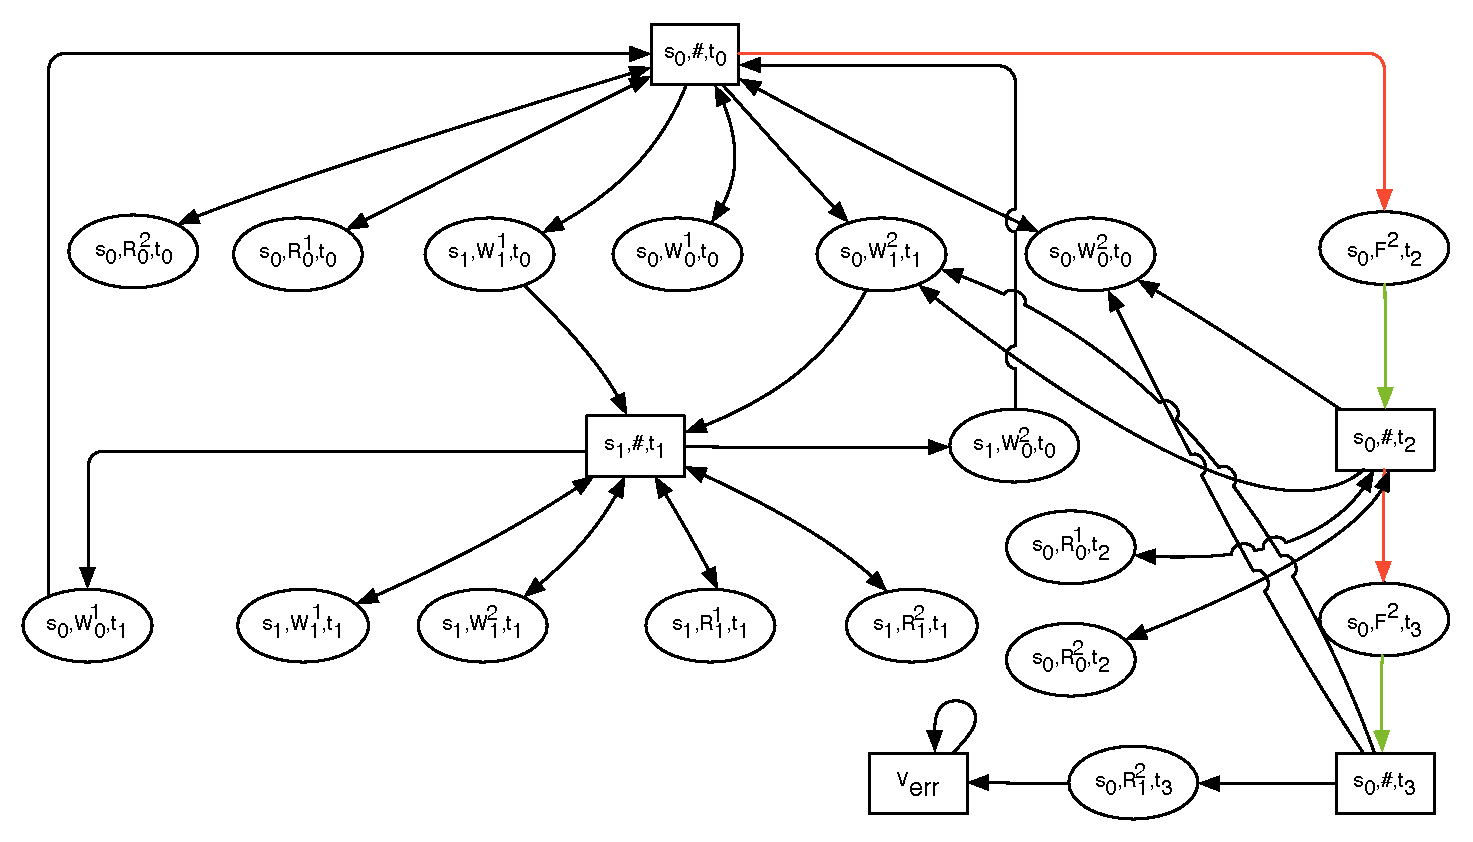
\includegraphics[scale=0.5]{Figs/ex1_cell_mem_game_graph_two_faults-eps-converted-to.pdf} 
  %  \vspace{-0.7cm}
%    \caption{Parte del grafo de juego de masking para la celda de memoria con dos fallas}
%    \label{figure:exam_2_mem_cell_gg_two_faults}
     %\vspace{-0.6cm}
%\end{center}
%\end{figure}

\begin{figure} [ht]
\begin{center}
  %% %\vspace{-0.5cm}
  %% % \includegraphics[scale=0.5]{ex1_cell_mem_game_graph_two_faults.eps} 
  %% \includegraphics[scale=0.5]{ex1_cell_mem_game_graph_two_faults.eps}
  %% %  \vspace{-0.7cm}

  \scalebox{0.8}{
  \begin{tikzpicture}[on grid,auto,align at top,
      hv path/.style={to path={-| (\tikztotarget)},rounded corners},
      vh path/.style={to path={|- (\tikztotarget)},rounded corners},
      hvh path/.style={to path={-- ++(#1,0) |- (\tikztotarget)},rounded corners}]
    
    \node[rvert] (s0xxxt0)                        {\makebox[4em][c]{$s_0,\#,t_0$}};

    \node[vvert] (s0w01t0) [below=2.2 of s0xxxt0] {\makebox[4em][c]{$s_0,w_0^1,t_0$}};
    \node[vvert] (s1w11t0) [left=2.0 of s0w01t0]  {\makebox[4em][c]{$s_1,w_1^1,t_0$}};
    \node[vvert] (s0r01t0) [left=2.0 of s1w11t0]  {\makebox[4em][c]{$s_0,r_0^1,t_0$}};
    \node[vvert] (s0r02t0) [left=2.0 of s0r01t0]  {\makebox[4em][c]{$s_0,r_0^2,t_0$}};
    \node[vvert] (s0w12t1) [right=2.0 of s0w01t0] {\makebox[4em][c]{$s_0,w_1^2,t_1$}};
    \node[vvert] (s0w02t0) [right=2.0 of s0w12t1] {\makebox[4em][c]{$s_0,w_0^2,t_0$}};
    \node[vvert] (s0ff2t2) [right=2.0 of s0w02t0] {\makebox[4em][c]{$s_0,F^2,t_2$}};

    \node[vvert] (s1w02t0) [below=2.2 of s0r02t0] {\makebox[4em][c]{$s_1,w_0^2,t_0$}};
    \node[rvert] (s1xxxt1) [below=2.2 of s1w11t0] {\makebox[4em][c]{$s_1,\#,t_1$}};
    \node[rvert] (s0xxxt2) [below=2.2 of s0ff2t2] {\makebox[4em][c]{$s_0,\#,t_2$}};

    \node[vvert] (s1w12t1) [below=2.2 of s1xxxt1] {\makebox[4em][c]{$s_1,w_1^2,t_1$}};
    \node[vvert] (s1w11t1) [left=2.0 of s1w12t1]  {\makebox[4em][c]{$s_1,w_1^1,t_1$}};
    \node[vvert] (s0w01t1) [left=2.0 of s1w11t1]  {\makebox[4em][c]{$s_0,w_0^1,t_1$}};
    \node[vvert] (s1r11t1) [right=2.0 of s1w12t1] {\makebox[4em][c]{$s_1,r_1^1,t_1$}};
    \node[vvert] (s1r12t1) [right=2.0 of s1r11t1] {\makebox[4em][c]{$s_1,r_1^2,t_1$}};
    \node[vvert] (s0r01t2) [right=2.0 of s0xxxt2] {\makebox[4em][c]{$s_0,r_0^1,t_2$}};

    \node[vvert] (s0ff2t3) [below=2.2 of s0xxxt2] {\makebox[4em][c]{$s_0,F^2,t_3$}};
    \node[vvert] (s0r02t2) [right=2.0 of s0ff2t3] {\makebox[4em][c]{$s_0,r_0^2,t_2$}};

    \node[rvert] (s0xxxt3) [below=2.2 of s0ff2t3] {\makebox[4em][c]{$s_0,\#,t_3$}};
    \node[vvert] (s0r12t3) [left=2.0 of s0xxxt3]  {\makebox[4em][c]{$s_0,r_1^2,t_3$}};
    \node[rvert] (verr)    [left=2.0 of s0r12t3]  {\makebox[4em][c]{$\ErrorSt$}};

    \path[{Latex[length=2.25mm,width=1.5mm]}-{Latex[length=2.25mm,width=1.5mm]},line width=0.7pt]
    (s0xxxt0) edge[bend right=15] (s0r02t0)
    (s0xxxt0) edge[bend right=10] (s0r01t0)
    (s0xxxt0) edge[]              (s0w01t0)
    (s0xxxt0) edge[bend left=10]  (s0w02t0)

    (s1xxxt1) edge[bend right=5]  (s1w11t1)
    (s1xxxt1) edge[]              (s1w12t1)
    (s1xxxt1) edge[bend left=5]   (s1r11t1)
    (s1xxxt1) edge[bend left=10]  (s1r12t1)
    (s0xxxt2) edge[]              (s0r01t2)
    (s0xxxt2) edge[]              (s0r02t2)
    ;

    \path[-{Latex[length=2.25mm,width=1.5mm]},line width=0.7pt]
    (s0xxxt0) edge[bend right=5]  (s1w11t0)
    (s0xxxt0) edge[bend left=5]   (s0w12t1)
    (s0xxxt0) edge[red,hv path]   (s0ff2t2)
    
    (s1w11t0) edge[]              (s1xxxt1)
    (s0w12t1) edge[bend left=10]  (s1xxxt1)
    (s0ff2t2) edge[darkgreen]     (s0xxxt2)

    (s1xxxt1) edge[bend right=10] (s0w01t1)
    (s1xxxt1) edge[]              (s1w02t0)
    (s1w02t0.west) edge[hvh path=-3mm]  ($(s0xxxt0.west) + (0,1mm)$)
    (s0xxxt2) edge[bend left=5]   (s0w02t0)
    (s0xxxt2) edge[bend left=10]  (s0w12t1)
    (s0xxxt2) edge[red]           (s0ff2t3)

    (s0w01t1.west) edge[hvh path=-5mm]  ($(s0xxxt0.west) + (0,2.5mm)$)
    (s0ff2t3) edge[darkgreen]     (s0xxxt3)

    (s0xxxt3) edge[bend left=15]  (s0w02t0)
    (s0xxxt3) edge[bend left=20]  (s0w12t1)
    (s0xxxt3) edge[]              (s0r12t3)
    (s0r12t3) edge[]              (verr)
    (verr)    edge[loop,out=195,in=165,looseness=7] (verr)
    ;

  \end{tikzpicture}
  }
    
  \caption{Parte del grafo de juego de enmascaramiento para la celda de memoria con dos fallas.}
  \label{figure:exam_2_mem_cell_gg_two_faults}
  %\vspace{-0.6cm}
\end{center}
\end{figure}

Los juegos de alcanzabilidad se pueden solucionar computando conjuntos $\text{Reach}_0$ (estados ganadores para el Refutador) como un punto fijo de conjuntos $\text{Reach}^i_0$  \cite{Jurd11}.
Estas ideas pueden ser adaptadas a nuestro contexto para tener en cuenta la cantidad de fallas. Esto sera útil en las próximas secciones, donde la cantidad de fallas es importante para razonar sobre la versión cuantitativa de los juegos de enmascaramiento.
\begin{definition}\label{def:U} Dado un grafo de juego de enmascaramiento fuerte $\StrMaskGG$, 
los conjuntos $\setsUs$ (para $i,j \geq 0$) se definen de la siguiente manera:
\begin{align*}
  U^0_i =& U^j_0 = \emptyset,  \label{def:of:Uji} \\
  U_1^1 =&  \{\ErrorSt\},
  \hspace{12.5cm} {}\notag
\end{align*}
\vspace{-0.97cm}
\begin{align*}
  U_{i+1}^{j+1} =&
    \{v' \mid v' \in V_\Refuter \wedge \post(v') \cap U_{i+1}^j \neq \emptyset\} \\
    &\textstyle\cup
    %\{v' \mid v' \in S_V \wedge post(v') \subseteq \bigcup_{j'\leq j} U_{i+1}^{j'} \wedge post(v') \cap U^j_{i+1} \neq \emptyset \wedge \pr{2}{v'} \notin \Faults \} \\
    %NOTE: above is the original condition of TACAS paper
    \{v' \mid v' \in V_\Verifier \wedge \post(v') \subseteq \bigcup_{i'\leq i+1, j' \leq j}U_{i'}^{j'} \\
    &\phantom{==}\wedge \post(v') \cap U^j_{i+1} \neq \emptyset \wedge \pr{1}{v'} \notin \Faults \} \\
    &\textstyle \cup
    \{v' \mid  v' \in V_\Verifier \wedge \post(v') \subseteq \bigcup_{i'\leq i, j' \leq j}U_{i'}^{j'} \\
    &\phantom{==}\wedge \post(v') \cap \setsUs \neq \emptyset \wedge \pr{1}{v'} \in \Faults \}
    \hspace{12.5cm} {}\notag
\end{align*}
Además, $U^k = \bigcup_{i \geq 0} U_i^k$ y $U = \bigcup_{k \geq 0} U^k$.
\end{definition}
Intuitivamente, el subíndice $i$ en $U^k_i$ indica que $\ErrorSt$ es alcanzado después de que hayan ocurrido a lo sumo $i-1$ fallas y $k$ pasos.
El siguiente lema se demuestra de forma directa utilizando técnicas estándar de juegos de alcanzabilidad \cite{AlfaroHK07}.
Notemos que estos conjuntos también pueden ser computados para juegos débiles de forma similar utilizando la relación $\Rightarrow$.
\begin{lemma} \label{lm:RefWinStrat} El Refutador tiene una estrategia ganadora en $\mathcal{G}_{A, A'}$ (o $\mathcal{G}^W_{A, A'}$) si y solo si $\InitVertex^G \in U^k$, para algún $k$.
\end{lemma}

% PRUEBA PASADA AL APENDICE
\iffalse
\begin{proof} 
``solo si'': La prueba utiliza resultados estándar de juegos de alcanzabilidad. Mas específicamente, considere el conjunto $V^G \setminus U$, este conjunto es una trampa para el Refutador, es decir, si $(s,\sigma, s', \Verifier) \in V^G \setminus U$, entonces existe un $v \in \post((s,\sigma, s', \Verifier))$ tal que 
$v \in V^G \setminus U$, sino
$(s,\sigma, s', \Verifier) \in U^k$ para algún $k$. Similarmente, si $(s,\#, s', R) \in V^G \setminus U$, entonces para todo $v \in \post((s,\#, s', \Refuter))$ 
tenemos $v \in V^G \setminus U$. Esto significa que $V^G \setminus U$ es una ``trampa'' para el Refutador. 
Ahora bien, podemos definir una estrategia para el Verificador $\pi_\Verifier$ de la siguiente manera: si $(s, \sigma, s', \Verifier) \in V^G \setminus U$, entonces
$\pi_\Verifier(s, \sigma, s', \Verifier) = \rho$ para algún $v \in V^G \setminus U$ el (cuya existencia esta garantizada), de lo contrario retorna un nodo arbitrario. 
Esta estrategia es ganadora para el Verificador desde cualquier $v \in V^G$, es decir, para cualquier jugada $\rho_0 \rho_1 \rho_2 \dots$ 
si $\rho_0 \in V^G \setminus U$, entonces $\forall i \geq 0: \rho_i \in V^G \setminus U$ 
(lo cual implica que $\forall i \geq 0: \rho_i \neq \ErrorSt$). 
La prueba es por inducción sobre $i$. Para $i=0$ el resultado es directo ya que $\rho_0 \in V^G \setminus \{\ErrorSt\}$. Para el caso inductivo,
supongamos que $\rho_i \in V^G \setminus U$. En el caso de que $\rho_i = (s, \sigma, s', \Verifier)$, entonces por definición de $\pi_\Verifier$, 
$\rho_{i+1} = \pi_\Verifier(s,\sigma, s', \Verifier) \in V^G \setminus U$.
Además, si $\rho_i = (s, \#, s', \Refuter)$, entonces $\post((s, \#, s', \Refuter)) \subseteq V^G \setminus U$, 
y por lo tanto $\rho_{i+1} \notin U$. 
Ahora bien, como $\InitVertex^G \notin U^k$ para todo $k$, entonces $\InitVertex^G \notin U$ y $\InitVertex^G \in V^G \setminus U$. 
En consecuencia, por la propiedad demostrada arriba $\Refuter$ tiene una estrategia ganadora desde 
$\InitVertex^G$. Pero esto es una contradicción porque el Refutador y el Verificador no pueden tener ambos estrategias ganadoras desde los mismos estados.
Por consiguiente, $\InitVertex^G \in U^k$ para algún $k$.
	
``si'': Considere $\InitVertex^G \in U^k$ para algún $k$, es decir, tenemos  $\InitVertex^G \in U^k_i$ para algún $i$ por Definición~\ref{def:U}. 
Además, para cada $v \in V^G$ definimos $\delta(v) = \min \{ (i,j) \mid v \in U^j_i \}$ (usando orden lexicográfico), por conveniencia asumimos $\min \emptyset = (\infty, \infty)$.
Entonces, la estrategia ganadora $\pi_R$ para el Refutador se define de la siguiente forma. Si $\delta(v) = (i,j)$ (con $(i,j) < (\infty, \infty)$), entonces $\pi_\Verifier(v) = w$, con $w$ siendo un vértice tal que
$\delta(w) = (i,j-1)$ (si $\pr{1}{v} \notin \Faults$) o $\delta(w) = (i-1,j-1)$ (si $\pr{1}{v} \in \Faults$), cuya existencia esta garantizada por Definición~\ref{def:U}. De otra forma, $\pi_\Refuter(v)$ retorna
un vértice arbitrario. Note que para cualquier jugada $\rho_0 \rho_1 \rho_2 \dots$ comenzando en $\InitVertex^G$ tenemos que:  para todo $i \geq 0$, $\delta(\rho_i) > \delta(\rho_{i+1})$, en orden lexicográfico.
Por lo tanto, para algún $k>0$ tenemos $\delta(\rho_k) = (1,1)$, y por tanto $\rho_k = \ErrorSt$.
\qedhere
\end{proof} \\
\fi

Por el Teorema \ref{thm:weak_thm}, esta prueba también aplica al juego de enmascaramiento débil $\WeakMaskGG$.
%By theorem \ref{thm:weak_thm}, the proof also applies for the weak masking game graph $\mathcal{G}^W_{A, A'}$. 
\section{Enmascaramiento Cuantitativo} \label{sec:QuantMask_mask}
En esta sección, extendemos el juego de simulación de enmascaramiento fuerte (resp. débil) introducido anteriormente con objetivos cuantitativos para así definir la noción de distancia de tolerancia a fallas enmascarante.
% In practice, fault-tolerance appears with a quantitative flavor, that is, fault-tolerant systems have %degrees of tolerance. This is particularly true when techniques like redundancy and voting are used.  %take this into account. 
Es importante remarcar que en este capítulo utilizamos el atributo  ``cuantitativo'' en un sentido no probabilista.
\begin{definition}  
  %Let $A=\langle S, \Sigma, E, s_0\rangle$ and $A'=\langle S', \Sigma_{\Faults}, E', s'_0 \rangle$.  T
  Para los sistemas de transición $A$ y $A'$, el \emph{grafo de juego de enmascaramiento cuantitativo fuerte} 
  $\QMStrGame = \langle V^G, V_\Refuter, V_\Verifier, E^G,  \InitVertex^G,  \reward^G \rangle$ se define de la siguiente manera:
 
\begin{itemize}
\item
  $\mathcal{G}_{A, A'}=\langle V^G, V_\Refuter, V_\Verifier, E^G, \InitVertex^G \rangle$ se define como en Definición~\ref{def:strong_masking_game_graph},
\item
  $ \reward^G(v) = (\chi_{\Faults}(\pr{1}{v}), \chi_{\ErrorSt}(v))$

\end{itemize}
%
donde $\chi_{\Faults}$ es la función característica sobre el conjunto $\Faults$, devolviendo $1$ si $\sigma \in \Faults$ y $0$ de otro modo, y $\chi_{\ErrorSt}$ es la función característica sobre el conjunto unitario $\{\ErrorSt\}$.
\end{definition}
Observemos que la función de recompensa retorna un par de números en lugar de un solo número. Es directo codificar al par como un único numero pero no lo hacemos por claridad. Remarcamos que el
\emph{grafo de juego de enmascaramiento cuantitativo débil} $\QMWeakGame$
se define de la misma forma que el grafo de juego definido arriba pero utilizando el grafo de juego de enmascaramiento débil $\mathcal{G}^W_{A, A'}$ en lugar de 
$\mathcal{G}_{A, A'}$


Dado un grafo de juego de enmascaramiento cuantitativo fuerte con la función de recompensa $\reward^G$ y la jugada 
$\rho = \rho_0 \rho_1 \rho_2, \ldots$, para todo $i \geq 0$, sea 
%$v_i = v^G(\rho_i \xrightarrow{\sigma_i} \rho_{i+1})$.
$r_i = \reward^G(\rho_i)$.
Definimos la \emph{función de payoff de enmascaramiento} de la siguiente manera: 
\[%\displaystyle
\FMask(\rho) = \lim_{n \rightarrow \infty}  \frac{\pr{1}{r_n}}{1+ \sum^{n}_{i=0} \pr{0}{r_i}},
%\FMask(\rho) = \liminf_{n \rightarrow \infty}  \frac{\pr{1}{v_n}}{1+ \sum^{n}_{i=0} \pr{0}{v_i}},
\]
la cual es proporcional a la inversa de la cantidad de movimientos de enmascaramiento realizados por el Verificador. Para entender esto, notemos que el numerador de $\frac{\pr{1}{r_n}}{1+ \sum^{n}_{i=0} \pr{0}{r_i}}$ será $1$
cuando alcancemos el estado de error, es decir, en aquellos caminos que no alcancen el estado de error esta fórmula devuelve $0$. Además, si el estado de error es alcanzado,  el denominador contará el número de transiciones de falla tomadas hasta el estado de error. Todas, a excepción de la última fueron enmascaradas exitosamente. Sin embargo, la última falla tratara de ser enmascarada por el Verificador, pero eventualmente llevará al estado de error.
Es decir, los vértices con valor $(1,\_)$ son aquellos correspondientes a fallas. Los demás se corresponden con $(0,\_)$.
Observemos también que si $\ErrorSt$ es alcanzado en $v_n$ sin la ocurrencia de ninguna falla, la parte nominal de la implementación no se corresponde con la especificación nominal, en cuyo caso $\frac{\pr{1}{r_n}}{1+ \sum^{n}_{i=0} \pr{0}{r_i}}=1$.
Entonces, el Refutador quiere maximizar el valor de cualquier jugada, es decir, tratará de alcanzar al estado $\ErrorSt$ bajo la menor cantidad de fallas, y por lo tanto enmascaramientos, posibles. 
Por el contrario, el Verificador quiere evitar $\ErrorSt$ y entonces tratará de enmascarar fallas de tal forma que se aleje del estado de error. 

Formalmente, el valor del juego de enmascaramiento cuantitativo fuerte para el Refutador se define como $\val_\Refuter(\QMStrGame) = \Sup_{\pi_\Refuter \in \Pi_\Refuter} \; \Inf_{\pi_\Verifier \in \Pi_\Verifier} \FMask(\out(\pi_\Refuter, \pi_\Verifier))$. De forma análoga, el valor del juego para el Verificador se define como $\val_\Verifier(\QMStrGame) = \Inf_{\pi_\Verifier \in \Pi_\Verifier} \; \Sup_{\pi_\Refuter \in \Pi_\Refuter} \FMask(\out(\pi_\Refuter, 
\pi_\Verifier))$. Entonces, definimos el valor del juego de enmascaramiento cuantitativo fuerte, denotado por $\val(\QMStrGame)$, como el valor del juego del Refutador o del Verificador, es decir, $\val(\QMStrGame) = \val_\Refuter(\QMStrGame) = \val_\Verifier(\QMStrGame)$. Esto es posible debido a que los juegos de enmascaramiento cuantitativos fuertes están determinados como lo probaremos mas adelante en el Teorema~\ref{thm:mask_game_det}. \\

\begin{definition} \label{def:mask_dist}
 Sean $A$ y $A'$ unos sistemas de transición. 
La \emph{distancia de enmascaramiento fuerte} entre $A$ y $A'$, denotada por $\DeltaMask(A, A')$ se define de la siguiente manera:
$\DeltaMask(A, A') = \val(\QMStrGame).$
\end{definition}

Es necesario remarcar que la \emph{distancia de enmascaramiento débil} $\DeltaMask^W$ se define de la misma forma para el grafo de juego de enmascaramiento cuantitativo débil $\QMWeakGame$.  A grandes rasgos, estamos interesados en medir la cantidad de fallas que pueden ser enmascaradas. El valor del juego está esencialmente determinado por las transiciones de falla en el grafo de juego y por cómo los jugadores pueden encontrar una estrategia que lleve a (o evite) el estado $\ErrorSt$, independientemente de la existencia de acciones silenciosas.

A continuación, estableceremos algunas propiedades básicas de este tipo de juegos. 
Como ya anticipamos, los juegos de enmascaramiento cuantitativos fuertes están determinados.

\begin{theorem} \label{thm:mask_game_det}
  Para cualquier grafo de juego de enmascaramiento cuantitativo fuerte $\QMStrGame$ con función de \textit{payoff} $\FMask$:
%  \vspace{-0.3cm}
  \[\textstyle
  \Inf_{\pi_\Verifier \in \Pi_\Verifier} \; \Sup_{\pi_\Refuter \in \Pi_\Refuter} \FMask(\out(\pi_\Refuter, \pi_\Verifier)) = \Sup_{\pi_\Refuter \in \Pi_\Refuter} \;  \Inf_{\pi_\Verifier \in \Pi_\Verifier} \FMask(\out(\pi_\Refuter, \pi_\Verifier))\]
\end{theorem}
\begin{proof} Para demostrar que la función de \textit{payoff} de enmascaramiento $\FMask$ está determinada tenemos que probar que está acotada y que es Borel-medible (teorema de Martin \cite{Martin98}). Primero, $\FMask$ está acotada por definición. Segundo, para ver que $\FMask$ es Borel-medible notemos que $\FMask(\Omega) \subseteq [0,1]$, y entonces es suficiente para probar que, para cada racional $x$, $\FMask^{-1}((-\infty, x])$ es Borel en la topología de Cantor de ejecuciones infinitas. 
Consideremos $\FMask^{-1}([-\infty,x])$ para un $x$ arbitrario, esto es lo mismo que $\FMask^{-1}([0, \frac{1}{a}])$ para un $a$ dado. Pero, $\FMask^{-1}([0, \frac{1}{a}]) = \bigcup_{b \geq a} A_b$ donde
$A_b = \bigcup_{i >0} A^i_b$ para $A^i_b = \{ \rho_0 \rho_1 \dots \mid \rho_i = \ErrorSt \wedge \sum^{i-1}_{j=0} \chi_{\Faults}(\pr{1}{\rho_j}) =b\}$. Notemos que 
$A^i_b = \{ C_{\rho_0 \dots \rho_i} \mid \sum^{i-1}_{j=0} \chi_{\Faults}(\pr{1}{\rho_j}) =b\}$ donde $C_{\rho_0 \dots \rho_i}$ es el cono correspondiente al segmento inicial 
$\rho_0 \dots \rho_i$ el cuál es Borel-medible, y por lo tanto $A^i_b$, $A_b$ y $\FMask^{-1}((-\infty, x])$ son Borel-medibles.
\qedhere
%is the set of all sequences $x_0 x_1 x_2 \dots$
%such that we have $b$ or more ones, and this is the union $\bigcup A_i$ being $A_i = \{\sigma \mid \mbox{ number of ones of } \sigma[0,i] = b\}$, which are Borel sets, thus $A$ is a Borel set.
\end{proof} \\


\subsection{Cómputo de la Distancia de Enmascaramiento}

En esta subsección presentamos los algoritmos para computar la distancia de enmascaramiento para un juego de enmascaramiento cuantitativo fuerte (resp. débil). Mostramos que, en el caso de sistemas deterministas, computar la distancia de enmascaramiento puede ser logrado utilizando un algoritmo de camino más corto. A diferencia de los sistemas no deterministas, en cuyo caso el cómputo puede ser realizado por un algoritmo de punto fijo.

Comenzamos presentando el próximo teorema que establece como se calcula el valor de un juego de enmascaramiento cuantitativo fuerte dado.
%

\begin{theorem} \label{thm:quant_game}
  Sea $\QMStrGame$ un grafo de juego de enmascaramiento cuantitativo fuerte.
  \sloppy Entonces, $\val(\QMStrGame) = \frac{1}{\pr{0}{\delta(\InitVertex^G)}}$, con
  $\delta(\InitVertex^G) = \min \{ (i,j) \mid  \InitVertex^G \in \setsUs \}$, siempre que
  $\InitVertex^G \in U$, y $\val(\QMStrGame)=0$ de otro modo, donde los conjuntos
   $\setsUs$ y $U$ están definidos en Definición~\ref{def:U}.

\end{theorem}
% PRUEBA PASADA AL APENDICE
\iffalse
\begin{proof} La prueba es por casos:
	
	Si $\InitVertex^G \notin U$, entonces definimos la siguiente estrategia para el Verificador. Si $v \in V_\Verifier \setminus U$, entonces $\pi^*_\Verifier(v)=v'$ 
	para algún $v' \in V_\Refuter \setminus U$, y si $v \notin  V_\Verifier \setminus U$, entonces $\pi^*_\Verifier(v) = v'$ para un $v'$ arbitrario. 
	Probamos por inducción que para cualquier jugada que se conforme a $\pi^*_\Verifier$: $\rho =\rho_0 \rho_1 \dots$ tenemos $\forall i \geq 0: \rho_i \notin V \setminus U$. El caso base es directo. 
Para el caso inductivo, asumamos que $\rho_i \notin V \setminus U$. En caso que $\rho_i \in V_\Verifier$, la propiedad se deduce por definición de
$\pi^*_\Verifier$. Si $\rho_i \in V_\Refuter$, como $\rho_i \in V^G \setminus U$, entonces $\post(\rho_i) \subseteq V^G \setminus U$ (por Definición~\ref{def:U}). 
Por lo tanto, $\rho_{i+1} \in V^G \setminus U$. 
	 Además, también tenemos $\rho_i \neq \ErrorSt$ ya que $\{ \ErrorSt \} \subseteq U$. También note que cualquier jugada que evite el estado $\ErrorSt$ tiene valor $0$: por definición de $\QMStrGame$, cada transición ejecutada por el Refutador debe ser sucedida por una transición seleccionada por el Verificador. Estas transiciones (las elegidas por el Verificador) tienen costo $(1,0)$ ya que el destino de cualquiera de estas transiciones es diferente de $\ErrorSt$. Como tenemos una cantidad infinita de estos movimientos del Verificador, cuando el estado $\ErrorSt$ no es alcanzado, la valuación de estas jugadas es $\lim_{n\rightarrow \infty} \frac{0}{1+ \sum^n_{i=0} \pr{0}{r_i}} = 0$ (recordemos que $r_i = \reward^G(\rho_i)$). 
En resumen, $\sup_{\pi_\Refuter \in \Pi_\Refuter} \FMask(\out(\pi_\Refuter, \pi^*_\Verifier)) = 0$, y como $\FMask$ es positiva
tenemos $\val(\QMStrGame) = \inf_{\pi_\Verifier \in \Pi_\Verifier} \sup_{\pi_\Refuter \in \Pi_\Refuter} \FMask(\out(\pi_\Refuter, \pi_\Verifier)) = 0$.

	Si $\InitVertex^G \in U$, tenemos que $\delta(\InitVertex^G) < (\infty, \infty)$, entonces definimos la siguiente estrategia para el Refutador. 
	Si $v \in U$, entonces $\pi^*_\Refuter(v)= v'$, donde $\delta(v') < \delta(v)$, sino $\pi^*_\Refuter(v)=v'$, para un $v'$ arbitrario. 
	La estrategia $\pi^*_R$ esta bien definida ya que si $v \in \setsUs$, entonces existe un $v' \in \post(v)$ tal que $v \in U^{j-1}_i$ (por Definición~\ref{def:U}). Además, $\delta(v') = (\pr{0}{\delta(v)}, \pr{1}{\delta(v)} - 1)$.  
	Ahora bien, probaremos que para cada estrategia $\pi_\Verifier \in \Pi_\Verifier$ tal que $\out(\pi^*_\Refuter, \pi_\Verifier) = \rho = \rho_0 \rho_1 \dots$ y $\rho_0 \in U$, tenemos:
\begin{equation}\label{eq:inf-bound}
	\FMask(\out(\pi^*_\Refuter, \pi_\Verifier)) \geq \frac{1}{ \pr{0}{\delta(\rho_0)}}
\end{equation} 
		Para demostrar esto, note que, si $\delta(\rho_0)= (i,j)$, entonces $\rho_j =\ErrorSt$ 
		ya que $\pr{1}{\delta(\rho_k)} = \pr{1}{\delta(\rho_{k+1})}+1$ para todo $k$. 
Esto significa que, en $j$ pasos tenemos $\delta(\rho_{j}) = (1,1)$ y entonces $\rho_{j} = \ErrorSt$.
	Esto implica que $\FMask(\rho) =  \lim_{n \rightarrow \infty}  \frac{\pr{1}{r_n}}{1+ \sum^{n}_{i=0} \pr{0}{r_i}} >0$, y también
$ \sum^{\pr{1}{\delta(\rho_0)} + k}_{i=0} \pr{0}{r_i} =  \sum^{\pr{1}{\delta(\rho_0)}}_{i=0} \pr{0}{r_i}$.
	 Es decir, probando que:
\begin{equation}\label{eq:bottom-sum}
 1+ \sum^{\pr{1}{\delta(\rho_0)}}_{i=0} \pr{0}{r_i} \geq \pr{0}{\delta(\rho_0)}
\end{equation} 
tenemos $\FMask(\rho) \geq \frac{1}{ \pr{0}{\delta(\rho_0)}}$. La prueba es por inducción sobre $\delta(\rho_0)$, el caso base es directo.
 Para el caso inductivo, si $\rho_0 \in V_\Refuter$, entonces
\begin{align*}
 	1 + \sum^{\pr{1}{\delta(\rho_0)}}_{i=0} \pr{0}{r_i} & =  1 + \pr{0}{r_0} + \sum^{\pr{1}{\delta(\rho_0)}}_{i=1} \pr{0}{r_i} & \\
					   %  & =   1+\sum^{\pr{1}{\delta(\rho_0)}}_{i=1} \pr{0}{r_i} & \\
					    % & =   1+\sum^{\pr{1}{\delta(\rho_1)}+1}_{i=1} \pr{0}{r_i} & \\
					     & =   1+ \sum^{\pr{1}{\delta(\rho_1)}}_{i=0} \pr{0}{r_{i+1}} &  \text{($\rho_0 \in V_\Refuter$)}\\
					     & \geq \pr{0}{\delta(\rho_1)} & \text{(I.H.)} \\
					     & = \pr{0}{\delta(\rho_0)} & \text{($\rho_0 \in V_\Refuter$)}
\end{align*}
 Si $\rho_0 \in V_\Verifier$ y $\pr{1}{\rho_0} \notin \Faults$, entonces la prueba es como arriba. Si $\pr{1}{\rho_0} \in \Faults$, entonces:
\begin{align*}
 	1+\sum^{\pr{1}{\delta(\rho_0)}}_{i=0} \pr{0}{r_i} & =  1+\pr{0}{r_0} + \sum^{\pr{1}{\delta(\rho_0)}}_{i=1} \pr{0}{r_i} & \\
					 %    & =   2 + \sum^{\pr{1}{\delta(\rho_0)}}_{i=1} \pr{0}{r_i} & \text{($\pr{1}{\rho_0} \in \Faults$)}\\
					  %   & =  2 +  \sum^{\pr{1}{\delta(\rho_1)}+1}_{i=1} \pr{0}{r_i} & \\
					     & =  2 +  \sum^{\pr{1}{\delta(\rho_1)}}_{i=0} \pr{0}{r_{i+1}} &   \text{($\pr{1}{\rho_0} \in \Faults$)}\\
					     & \geq 1 + \pr{0}{\delta(\rho_1)} & \text{(I.H.)} \\
					     & = \pr{0}{\delta(\rho_0)} & \text{($\pr{1}{\rho_0} \in \Faults$)}
\end{align*}
Por lo tanto, la inecuación \ref{eq:bottom-sum} vale. Ahora bien, consideremos la estrategia $\pi^*_\Verifier$ para el Verificador que se define a continuación. Para $v \in U$, $\pi^*_\Verifier(v) = v'$ tal que $\delta(v') = \max \{\delta(v'') \mid v'' \in \post(v)\}$, sino $\pi^*_\Verifier(v) = v'$ para un $v'$ arbitrario. 
Vamos a probar que $\FMask(\out(\pi^*_\Refuter, \pi^*_\Verifier)) = \frac{1}{\pr{0}{\delta(\rho_0)}}$. 
%Let $(\out(\pi^*_\Verifier, \pi^*_\Refuter)) = \rho_0 \rho_1 \dots$.
Note que, por definición de $\pi^*_\Verifier$ y $\pi^*_\Refuter$, tenemos que $\pr{1}{\delta(\rho_{i+1})} = \pr{1}{\delta(\rho_i)} - 1$, %$\pr{1}{\delta(\rho_i)} = \pr{1}{\delta(\rho_{i+1})}+1$
es decir, en a lo sumo $\pr{1}{\delta(\rho_0)}$ pasos alcanzamos $\ErrorSt$. De esta forma, $\lim_{n \rightarrow \infty}  \pr{1}{r_n} =1$. 
Además, si $\pr{1}{\rho_i} \in \Faults$, entonces $\pr{0}{\delta(\rho_{i+1})} = \pr{0}{\delta(\rho_i)} - 1$
por definición de $\pi^*_V$. De este modo, ocurrirán a lo sumo $\pr{0}{\rho_0}$ fallas en $\rho$, y entonces
$\FMask(\out(\pi^*_\Refuter, \pi^*_\Verifier)) = \frac{1}{\pr{0}{\delta(\rho_0)}}$. Por lo tanto, esto y la inecuación \ref{eq:inf-bound} nos da: 
$\inf_{\pi_\Verifier \in \Pi_\Verifier} \FMask(\out(\pi^*_\Refuter, \pi_\Verifier)) = \frac{1}{\pr{0}{\delta(v^G_0)}}$. 


Por último, demostraremos que no existe una estrategia $\pi^+_\Refuter$  de tal forma que $\sup_{\pi_\Verifier} \FMask(\out(\pi^+_\Refuter, \pi_\Verifier)) < \frac{1}{\pr{0}{\delta(v^G_0)}}$. 
De esta forma, $\pi^*_\Refuter$ es la mejor estrategia. 
Vamos a hacer una prueba por contradicción, asumamos que tenemos tal estrategia. Consideremos $\out(\pi^+_\Refuter, \pi^*_\Verifier) = \rho = \rho_0 \rho_1 \dots$, 
y sea $\delta(\rho_0) = (i,j)$. Entonces, note que, si $\rho_i \in V_\Refuter$, entonces $\pr{0}{\delta(\rho_i)} = \pr{0}{\delta(\rho_{i+1})}$, 
además, si $\rho_i \in V_\Verifier$ entonces $\pr{0}{\delta(\rho_i)} = 1 + \pr{0}{\delta(\rho_{i+1})}$. 
Por lo tanto, $\lim_{n \rightarrow \infty}\sum^n_{0} \pr{0}{r_i} = \frac{1}{\pr{0}{\delta(\rho_0)}}$, lo cual lleva a una contradicción.
Entonces, $\val(\QMStrGame) = \inf_{\pi_\Verifier \in \Pi_\Verifier} \sup_{\pi_\Refuter \in \Pi_\Refuter} \FMask(\out(\pi_\Refuter, \pi_\Verifier)) = \frac{1}{\pr{0}{\delta(v^G_0)}}$.
\qedhere
.

\end{proof} \\
\fi

Interesantemente, el valor del juego para juegos deterministas está dado por el camino más corto (si existe) hacia el estado de error, como se establece en el siguiente teorema.
\begin{theorem}\label{thm:det-games} Sea  $\QMStrGame = \langle V^G, V_\Refuter,V_\Verifier, E^G, \InitVertex^G, \reward^G \rangle$ un grafo de juego de enmascaramiento cuantitativo fuerte determinista,
y sea  $G_{\QMStrGame} = \langle V^G,  E^G, \InitVertex^G, w \rangle$ su grafo con pesos subyacente, con la función de peso $w$ 
definida como:
\[
w(v, v') =
\begin{cases} 1 & \text{si $\pr{1}{v'} \in \Faults$} \\
		      0 & \text{en caso contrario}	 
\end{cases}
\]
	Si $\rho = \rho_0 \rho_1  \dots \ErrorSt$ es el camino mas corto (con respecto a la función $w$)
hacia el estado de error en $G_{\QMStrGame}$, y $k$ es la cantidad de fallas que ocurren en $\rho$, entonces: 
\[
	\val(\QMStrGame) = \frac{1}{1+k}
\]
\end{theorem}
% PRUEBA PASADA AL APENDICE
\iffalse
\begin{proof}
	Definamos la estrategia $\pi_\Refuter \in \Pi_\Refuter$ para el Refutador tal que:
\[
	\inf_{\pi_\Verifier \in \Pi_\Verifier} f_m(\out(\pi_\Refuter, \pi_\Verifier)) = \sup_{\pi_\Refuter' \in \Pi_\Refuter} \inf_{\pi_\Verifier \in \Pi_\Verifier} f_m( \out(\pi_\Refuter',\pi_\Verifier))
\]	
	donde esta estrategia se conforma con el camino mas corto en el grafo subyacente. Asumamos que: 
$\rho_0 \rho_1 \dots \ErrorSt$ es el camino mas corto. Podemos asumir de forma segura que ningún vértice aparece mas de una vez en $\rho$, de lo contrario podemos reducir el camino mas corto eliminando ciclos.
	Teniendo en cuenta esto, definimos la estrategia $\pi_\Refuter$ de la siguiente forma:
\[
	\pi_\Refuter(v) = \begin{cases}
								\rho_{j+1} & \text{si $v = \rho_j$ para algún $j \geq 0$,} \\
								v' & \text{para un $v' \in V_\Verifier$ arbitrario.}
						   \end{cases}
\] 
Primero, vamos a probar que $\inf_{\pi_\Verifier \in \Pi_\Verifier} f_m (\out(\pi_\Refuter, \pi_\Verifier)) = \frac{1}{1+k}$. Sea $\pi_\Verifier$ una estrategia arbitraria para el Verificador. Probemos que la jugada $\rho'_0 \rho'_1 \dots$ que se conforma a $\pi_\Refuter$ y $\pi_\Verifier$ es igual a $\rho$. Esto lo demostramos por inducción sobre $\rho_i$, vale para $\rho_0 = \InitVertex = \rho'_0$. Asumamos que vale para $i=n$, es decir, $\rho'_n = \rho_n$, si $\rho_n = (t, \sigma^1, s', \Verifier)$ (resp.  $\rho_n = (s, \sigma^2, t', \Verifier)$), como $A$ y $A'$ son deterministas, existe un único arco $((t, \sigma^1, s', \Verifier), (t, \#, t', \Verifier)) \in E^G$ (resp. $((s, \sigma^1, t', \Verifier), (t, \#, t', \Verifier)) \in E^G$) y por lo tanto  $\rho'_{n+1} = \pi_\Verifier( \rho'_n) = (t, \#, t', \Verifier) = \rho_{n+1}$. Si 
$\rho'_n = \rho_n = (s, \#, s', \Refuter)$ entonces $\rho'_{n+1} = \pi_\Refuter(\rho'_n) = \pi_\Refuter(\rho_n) = \rho_{n+1}$. 
	
Adicionalmente, la valuación de $\rho$ es $\frac{1}{1+k}$, es decir, obtenemos:
\begin{equation} \label{eq1}
\begin{split}
 f_m (\out(\pi_\Refuter, \pi_\Verifier))  =  \frac{1}{1+k},
\end{split}
\end{equation}	
y como esto vale para cualquier $\pi_\Verifier$, obtenemos:
\begin{equation} \label{eq2}
\begin{split}
\inf_{\pi_V \in \Pi_V} f_m (\out(\pi_\Refuter, \pi_\Verifier))  =  \frac{1}{1+k}
\end{split}
\end{equation}

Ahora bien, asumamos que hay una estrategia $\pi_\Refuter'$ para el Refutador tal que 
$\inf_{\pi_V \in \Pi_V} f_m (\out(\pi_\Refuter', \pi_\Verifier)) > \inf_{\pi_\Verifier \in \Pi_\Verifier} f_m (\out(\pi_\Refuter, \pi_\Verifier))$.
De (\ref{eq1}) tenemos que $\inf_{\pi_\Verifier \in \Pi_\Verifier} f_m(\out(\pi_\Refuter', \pi_\Verifier)) > \frac{1}{1+k}$. 
De esta forma, la cantidad de fallas observadas en 
$\inf_{\pi_\Verifier \in \Pi_\Verifier} f_m(\out(\pi_\Refuter', \pi_\Verifier))$ debería ser menor a $k$. 
Pero, seria un camino mas corto en el grafo subyacente, lo cual es una contradicción. Por lo tanto, tenemos que:
\[	
	\inf_{\pi_\Verifier \in \Pi_\Verifier} f_m(\out(\pi_\Refuter, \pi_\Verifier)) = \sup_{\pi_\Refuter' \in \Pi_\Refuter} \inf_{\pi_\Verifier \in \Pi_\Verifier} f_m( \out(\pi_\Refuter',\pi_\Verifier)).
\]	
\qedhere
\end{proof} \\
\fi

Notemos que los Teoremas~\ref{thm:mask_game_det}, \ref{thm:quant_game} y \ref{thm:det-games} aplican también a 
$\QMWeakGame$.
El Teorema~\ref{thm:det-games} nos permite proveer procedimientos eficientes para decidir juegos cuantitativos en el caso de sistemas deterministas. Para el caso de sistemas no deterministas, el procedimiento es más costoso en cuanto a recursos computacionales (en términos de tiempo y memoria) que para el caso de sistemas deterministas, ya que es necesario computar los conjuntos $\setsUs$ (Definición~\ref{def:U}). \\

Es importante destacar que, para sistemas no deterministas, el camino más corto no siempre determina estrategias ganadoras. Esto se puede observar a continuación a través de un ejemplo simple. Consideremos los dos sistemas de transición que se muestran en la Figura~\ref{fig:two-nondet-systems}.


\begin{figure}
\begin{center}
\scalebox{1.2}{
\begin{subfigure}{.32\textwidth}\centering
  \begin{tikzpicture}[on grid,auto,align at top]
    \node[state] (n0)                   {$s_0$};
    \node[state] (n1) [below=1.2 of n0] {$s_1$};
    \node[state] (n2) [right=1.6 of n1] {$s_2$};
    \node[state] (n3) [below=1.2 of n1] {$s_3$};

    \path[-Latex]
    (n0) edge[]  node {$a$}   (n1)
    (n1) edge[] node[swap] {$b$} (n2)
    (n1) edge[] node {$b$} (n3)
    (n2) edge[bend right=25] node[swap] {$d$} (n0)
    (n3) edge[bend left=35] node {$e$} (n0)
    ;
  \end{tikzpicture}
  \caption{M}
  \end{subfigure}
  \begin{subfigure}{.32\textwidth}\centering
  \begin{tikzpicture}[on grid,auto,align at top]
    \node[state] (n0)                   {$t_0$};
    \node[state] (n1) [below=1.2 of n0] {$t_1$};
    \node[state] (n2) [right=1.6 of n1] {$t_2$};
    \node[state] (n3) [below=1.2 of n1] {$t_3$};

    \path[-Latex]
    (n0) edge[]  node {$a$}   (n1)
    (n1) edge[] node[swap] {$b$} (n2)
    (n1) edge[] node {$b$} (n3)
    (n2) edge[bend right=25] node[swap] {$d$} (n0)
    (n3) edge[bend left=35] node {$e$} (n0)
    (n2) edge[red,bend left=25] node {$F$} (n3)
    ;
  \end{tikzpicture}
  \caption{M'}
  \end{subfigure}
  }
  \caption{Dos sistemas no deterministas.}
    \label{figure:nondeterm}\label{fig:two-nondet-systems}
  \end{center}
  \end{figure}
  
%\begin{figure} [ht]
%\begin{center}
%    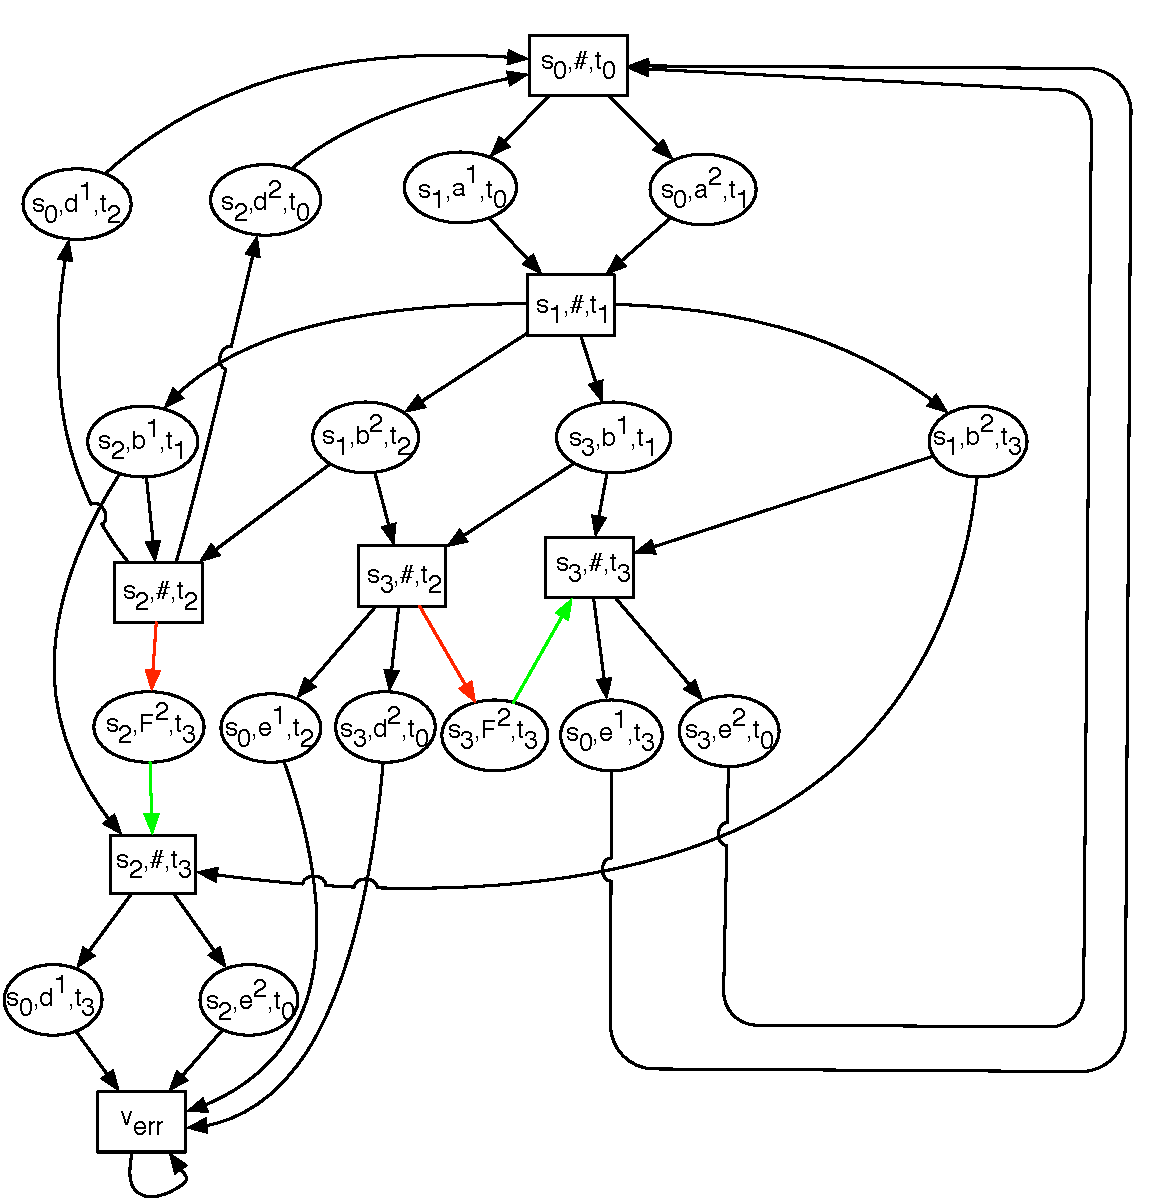
\includegraphics[scale=0.5]{Figs/nondeterm-game-eps-converted-to.pdf} 
%    \caption{Grafo de juego para M y M'}
%    \label{figure:nondeterm-game}
%%\end{figure}

\begin{figure} [ht]
\begin{center}
  %% %\vspace{-0.5cm}
  %% % \includegraphics[scale=0.5]{ex1_cell_mem_game_graph_two_faults.eps} 
  %% \includegraphics[scale=0.5]{ex1_cell_mem_game_graph_two_faults.eps}
  %% %  \vspace{-0.7cm}

  \scalebox{0.8}{
  \begin{tikzpicture}[on grid,auto,align at top,
      hv path/.style={to path={-| (\tikztotarget)},rounded corners},
      vh path/.style={to path={|- (\tikztotarget)},rounded corners},
      hvh path/.style={to path={-- ++(#1,0) |- (\tikztotarget)},rounded corners},
      vhv path/.style={to path={-- ++(0.4,0) |- (\tikztotarget)},rounded corners},
      4giros path/.style={to path={-- ++(0,-1) -- ++(3.5,0) -- ++(0,10.8) -|(\tikztotarget)},rounded corners},
      3giros path/.style={to path={-- ++(0,-0.5) |- ++(1,0) |- (\tikztotarget)},rounded corners}]
    
    \node[rvert] (s0xxxt0)                        {\makebox[4em][c]{$s_0,\#,t_0$}};

    \node[vvert] (s1a1t0) [below=1.7 of s0xxxt0] {\makebox[4em][c]{$s_1,a^1,t_0$}};
    \node[vvert] (s0a2t1) [right=2.0 of s1a1t0]  {\makebox[4em][c]{$s_0,a^2,t_1$}};
    \node[vvert] (s2d2t0) [left=2.0 of s1a1t0]  {\makebox[4em][c]{$s_2,d^2,t_0$}};
    \node[vvert] (s0d1t2) [left=2.0 of s2d2t0]  {\makebox[4em][c]{$s_0,d^1,t_2$}};

    \node[rvert] (s1xxxt1) [below=1.7 of s1a1t0]  {\makebox[4em][c]{$s_1,\#,t_1$}};

    \node[vvert] (s3b1t1) [below=1.7 of s1xxxt1]  {\makebox[4em][c]{$s_3,b^1,t_1$}};
    \node[vvert] (s1b2t3) [right=2.0 of s3b1t1]  {\makebox[4em][c]{$s_1,b^2,t_3$}};
    \node[vvert] (s1b2t2) [left=2.0 of s3b1t1]  {\makebox[4em][c]{$s_1,b^2,t_2$}};
    \node[vvert] (s2b1t1) [left=2.0 of s1b2t2]  {\makebox[4em][c]{$s_2,b^1,t_1$}};

    \node[rvert] (s3xxxt3) [below=1.7 of s1b2t3]  {\makebox[4em][c]{$s_3,\#,t_3$}};
    \node[rvert] (s3xxxt2) [left=2.0 of s3xxxt3]  {\makebox[4em][c]{$s_3,\#,t_2$}};
    \node[rvert] (s2xxxt2) [left=2.0 of s3xxxt2]  {\makebox[4em][c]{$s_2,\#,t_2$}};

    \node[vvert] (s3f2t3) [below=1.7 of s3xxxt3]  {\makebox[4em][c]{$s_3,F^2,t_3$}};
    \node[vvert] (s3d2t0) [left=2.0 of s3f2t3]  {\makebox[4em][c]{$s_3,d^2,t_0$}}; 
    \node[vvert] (s0e1t2) [left=2.0 of s3d2t0]  {\makebox[4em][c]{$s_0,e^1,t_2$}};
    \node[vvert] (s2f2t3) [left=2.0 of s0e1t2]  {\makebox[4em][c]{$s_2,F^2,t_3$}}; 
    \node[vvert] (s0e1t3) [right=2.0 of s3f2t3]  {\makebox[4em][c]{$s_0,e^1,t_3$}};
    \node[vvert] (s3e2t0) [right=2.0 of s0e1t3]  {\makebox[4em][c]{$s_3,e^2,t_0$}};

    \node[rvert] (s2xxxt3) [below=1.7 of s2f2t3]  {\makebox[4em][c]{$s_2,\#,t_3$}};

    \node[vvert] (s0d1t3) [below=1.7 of s2xxxt3]  {\makebox[4em][c]{$s_0,d^1,t_3$}};
    \node[vvert] (s2e2t0) [right=2.0 of s0d1t3]  {\makebox[4em][c]{$s_2,e^2,t_0$}};

    
    
    \node[rvert] (verr)    [below=1.7 of s2e2t0]  {\makebox[4em][c]{$\ErrorSt$}};

    \path[-Latex]
    (s0xxxt0) edge[] (s1a1t0)
    (s0xxxt0) edge[]  (s0a2t1)
    (s2d2t0) edge[]  (s0xxxt0)
    (s0d1t2) edge[]  (s0xxxt0)

    (s1a1t0) edge[]  (s1xxxt1)
    (s0a2t1) edge[]  (s1xxxt1)

    (s1xxxt1) edge[]  (s2b1t1)
    (s1xxxt1) edge[]  (s1b2t2)
    (s1xxxt1) edge[]  (s3b1t1)
    (s1xxxt1) edge[]  (s1b2t3)

    (s2b1t1) edge[bend right=35]  (s2xxxt3)
    (s2b1t1) edge[]  (s2xxxt2)
    (s1b2t2) edge[]  (s2xxxt2)
    (s1b2t2) edge[]  (s3xxxt2)
    (s3b1t1) edge[]  (s3xxxt2)
    (s3b1t1) edge[]  (s3xxxt3)
    (s1b2t3.east) edge[vhv path=-3mm]  (s2xxxt3)
    (s1b2t3) edge[]  (s3xxxt3)
    
    (s2xxxt2) edge[bend left=10]              (s0d1t2)
    (s2xxxt2) edge[bend right=35]              (s2d2t0)
    (s2xxxt2) edge[red]              (s2f2t3)
    (s3xxxt2) edge[]              (s0e1t2)
    (s3xxxt2) edge[]              (s3d2t0)
    (s3xxxt2) edge[red]              (s3f2t3)
    (s3xxxt3) edge[]              (s0e1t3)
    (s3xxxt3) edge[]              (s3e2t0)

    (s2f2t3) edge[darkgreen]              (s2xxxt3)
    (s0e1t2) edge[bend left=36]              (verr)
    (s3d2t0) edge[bend left=32]              (verr)
    (s3f2t3) edge[darkgreen]              (s3xxxt3)
    (s0e1t3.south) edge[4giros path=-3mm]              (s0xxxt0.north)
    (s3e2t0.south) edge[3giros path=-3mm]              (s0xxxt0)

    (s2xxxt3) edge[]              (s0d1t3)
    (s2xxxt3) edge[]              (s2e2t0)
    (s0d1t3) edge[]              (verr)
    (s2e2t0) edge[]              (verr)
    (verr) edge[loop,out=195,in=165,looseness=7]              (verr)
    ;

  \end{tikzpicture}
  }
    
  \caption{Grafo de juego para M y M'.}
  \label{figure:nondeterm-game}
  %\vspace{-0.6cm}
\end{center}
\end{figure}

En este ejemplo, el no-determinismo está dado por la acción $b$. También observemos que hay una falla en $M'$ que conecta los estados $t_2$ y $t_3$. El juego cuantitativo para estos sistemas se muestra en la Figura~\ref{figure:nondeterm-game}. Notemos que cualquier camino más corto en este grafo con respecto a la función de peso $w$ tiene valor $1$ (cualquier camino en el grafo que evite las fallas). Sin embargo, el valor del juego es $\frac{1}{2}$ ya que la mejor estrategia del Refutador es llevar al Verificador al estado $(s_2,b^1,t_1,\Verifier)$. 
Desde ahí, como el Verificador quiere minimizar el valor del juego, su mejor jugada es hacer un movimiento hacia el estado $(s_2,\#,t_2,\Refuter)$. Entonces, el Refutador puede elegir una falla que lleva al estado de error. \\
%Note that the value of this game is $\frac{1}{2}$.\\

La observación anterior sugiere que se necesita un algoritmo diferente para computar la distancia de enmascaramiento para sistemas no deterministas. 
La idea principal es computar los conjuntos $\setsUs$ que fueron definidos en Definición~\ref{def:U} a través de un algoritmo de punto fijo. Para ser más precisos, los conjuntos $\setsUs$ pueden ser calculados utilizando una búsqueda \textit{bottom-up breadth-first} (primero a lo ancho de abajo hacia arriba) desde el estado de error. 
El algoritmo \ref{Alg:MainAlg} muestra el pseudo-código para resolver cualquier juego cuantitativo de enmascaramiento fuerte (resp. débil). 
El algoritmo toma como entrada un grafo de juego cuantitativo de enmascaramiento fuerte  $\QMStrGame = \langle V^G, V_\Refuter, V_\Verifier,E^G, \InitVertex^G, \reward^G \rangle$ 
y computa el valor del juego, es decir, $\val(\QMStrGame)$.
%Let us describe the essential steps of the algorithm for solving any quantitative strong (resp. weak) masking game. 
El algoritmo etiqueta los nodos del grafo con los índices $i$ y $j$. 
%The algorithm can be understood as follows. 
Los pasos principales del algoritmo se detallan a continuación:


\begin{enumerate}
  \item Cada vértice $v$ está etiquetado con un par $(i, j)$ que representa que $v \in U_{i}^{j}$. Inicialmente, $\ErrorSt$ está etiquetado con $(1, 1)$ y todos los demás nodos están etiquetados con $(\infty, \infty)$ (lineas \ref{Alg:InitB}-\ref{Alg:InitE}). 
  Además, utilizamos la asignación $\Q \gets \emptyset$ para denotar la creación de una cola vacía. 
  Después, encolamos el estado de error (lineas \ref{Alg:CreateQ}-\ref{Alg:LoopB}). También mantenemos un conjunto $\STB$ que contiene los estados estabilizados, es decir estados cuyas etiquetas son finales. Los estados que no son alcanzables (hacia atrás) desde el estado de error son ignorados.
  \item Desde el estado de error se lleva a cabo una búsqueda a lo ancho de abajo hacia arriba utilizando una cola de prioridad $\Q$ (lineas \ref{Alg:LoopB}-\ref{Alg:LoopE}), donde el estado con la etiqueta más pequeña (considerando el orden lexicográfico) tiene mayor prioridad. 
  Sea $v'$ el vértice con la prioridad más alta en la cola. Entonces, para todo predecesor $v$ de $v'$ se ejecutan los siguientes pasos (lineas \ref{Alg:LoopBPre}-\ref{Alg:LoopEPre}):
  \begin{itemize}
    \item Si $v$ es un nodo del Verificador (resp. un nodo del Refutador), entonces obtenemos la máxima (resp. mínima) etiqueta $(i,j)$ de todos sus sucesores con respecto al orden lexicográfico. Adicionalmente, si $v$ es un vértice del Verificador y todos sus sucesores están en $\STB$, entonces $v$ se añade al conjunto. En el caso que $v$ sea un vértice del Refutador, 
    el vértice simplemente se añade sin restricción alguna. 
    \item Actualizar el valor de $(i,j)$ incrementando $j$, e incrementando $i$ solo si $\pr{1}{v} \in \Faults$. Llamemos $(i',j')$ a esta nueva etiqueta.
    \item Si $i'$ es diferente del primer componente de la etiqueta actual de $v$, entonces se actualiza y se agrega $v$ a la cola. 
    Observemos que el mismo nodo puede ser añadido a la cola más de una vez a medida que las etiquetas de sus sucesores cambian.
  \end{itemize}
  \item Cuando la cola está vacía, 
  el algoritmo termina y retorna el valor del juego (lineas \ref{Alg:EndB}-\ref{Alg:EndE}). 
  Intuitivamente, el procedimiento termina tan pronto como las etiquetas de todos los estados en el grafo de juego alcanzan su valor final (es decir se alcanza un punto fijo). 
  Sea $k$ la primer componente de la etiqueta del estado inicial, entonces el valor del juego es $\frac{1}{k}$ si 
  $\InitVertex^G \in \STB$, y $0$ en caso contrario.\\
\end{enumerate}
\begin{algorithm}[t!]
\SetAlgoLined
\KwIn{Juego de Enmascaramiento Cuantitativo Fuerte $\QMStrGame = \langle V^G, V_\Refuter, V_\Verifier,E^G, \InitVertex^G, \reward^G \rangle$}
\KwOut{$\val(\QMStrGame)$}
 Etiquetar $\ErrorSt$ con $(1,1)$\; \label{Alg:InitB}
 Etiquetar cada nodo en $V^G \setminus \{\ErrorSt\}$ con $(\infty,\infty)$\; \label{Alg:InitE}
 %$\Q \gets \emptyset$ \tcp*{$\Q$ is a priority queue}  \label{Alg:CreateQ}
 $\Q \gets \emptyset$ \tcp*{$\Q$ es una cola de prioridad}  \label{Alg:CreateQ}
 $\STB \gets \{\ErrorSt\}$\; \label{Alg:CreateSTB}
 %$\mathcal{VE} \longleftarrow \emptyset$\; \label{Alg:CreateVE} 

 $\enqueue(\Q, \ErrorSt)$\; \label{Alg:LoopB} 
 \While{$\Q$ no está vacía}{ \label{Alg:While} 
 	 $v' \gets \dequeue(\Q)$\; \label{Alg:Dequeue-Node}
 	 %\lIf{$\{s'\xrightarrow{\sigma}t \mid t \in post(s')\} \subseteq \mathcal{VE}$}{ \label{Alg:UpdateSTB}
	%	$\mathcal{STB} \longleftarrow \mathcal{STB} \cup \{s'\}$
	 %}
	 
	 \For{$v \in \pre(v') \wedge v \notin \STB$ }{ \label{Alg:LoopBPre}
	 %\For{$s\xrightarrow{\sigma}s' \in E^G$}{ \label{Alg:LoopBPre}
	 	\If{$v \in V_\Verifier$}{
	 		$\lbl \gets \maxlabel(\post(v))$\; \label{Alg:V-Update}
	 		\lIf{$\post(v) \subseteq \STB$}{ \label{Alg:UpdateSTB}
	 		$\STB \gets \STB \cup \{v\}$ 
	 		}
	 		%$enq \longleftarrow post(s) \subseteq \mathcal{STB}$
	 	}
	 	\Else{
	 		$\lbl \gets \minlabel(\post(v))$\; \label{Alg:R-Update}
	 		%$enq \longleftarrow post(s) \cap \mathcal{STB} \neq \emptyset$
	 		$\STB \gets \STB \cup \{v\}$ \label{Alg:R-STB-Update}
	 	}
	 	$\pr{1}{\lbl} \gets \pr{1}{\lbl} + 1$ \tcp*{asumimos $\infty+1=\infty$} \label{Alg:Inc_j}
	 	\lIf{$\pr{1}{v} \in \Faults$}{
	 		$\pr{0}{\lbl} \gets \pr{0}{\lbl} + 1$  \label{Alg:Inc_i}
	 	}
	 	\If{$\pr{0}{\Label(v)} \neq \pr{0}{\lbl}$}{ \label{Alg:Insert-Cond}
	 		Etiquetar $v$ con $\text{lbl}$\;
	 		$\text{Enqueue}(\Q, v)$  \tcp*{$v$ tiene prioridad $\Label(v)$} \label{Alg:Enqueue-Vertex}
	 		%$\mathcal{VE} \longleftarrow \mathcal{VE} \cup \{s\xrightarrow{\sigma}s'\}$
	 	}
	 } \label{Alg:LoopEPre}
 } \label{Alg:LoopE}
 %\lIf{$\pr{0}{Label(s_{0}^G)} \neq \infty$}{ \label{Alg:EndB}
 \lIf{$\InitVertex^G \in \STB$}{ \label{Alg:EndB}
	$\result \gets \frac{1}{\pr{0}{\Label(\InitVertex^G)}}$
 }
 \lElse{
	$\result \gets 0$ \label{Alg:Ret0}
 }
 \Return{$\result$}\; \label{Alg:EndE}
 \caption{Computando el valor del juego de enmascaramiento cuantitativo fuerte} \label{Alg:MainAlg} 
\end{algorithm}


	 Vamos a demostrar que el algoritmo termina y que es correcto.

\sloppy \begin{theorem}\label{thm:alg-termination}  \textbf{(Terminación)} El Algoritmo \ref{Alg:MainAlg} termina.
\end{theorem}
\begin{proof}
Probemos que un vértice no puede ser añadido una cantidad no acotada de veces a $\Q$. 
Primero, observemos que las lineas \ref{Alg:LoopBPre} y \ref{Alg:R-STB-Update} del Algoritmo  \ref{Alg:MainAlg} implican que los vértices del Refutador solo se agregan una vez a la cola. 
Por lo tanto, solo los vértices del Verificador pueden ser añadidos a a $\Q$ una cantidad no acotada de veces.
Probaremos por contradicción que este no es el caso. 
Asumamos que $v$ es un vértice del Verificador que es agregado infinitas veces a la cola. 
Esto implica que $v \notin \STB$ es siempre verdadero dentro del ciclo, y entonces 
$\post(v) \cap (V^G \setminus \STB) \neq \emptyset$ (d lo contrario $v$ seria insertado en $\STB$, linea \ref{Alg:UpdateSTB}). 
Esto significa que,  algún nodo $w \in \post(v)$ del Refutador debe satisfacer $\post(w) \cap \STB = \emptyset$. 
Mas aun, también tenemos $\Label(w) = (\infty, \infty)$ ya que este es el valor inicial que se asigna a $w$, 
y la única manera de modificarlo es ejecutando la linea \ref{Alg:R-Update}, 
en tal caso, $w$ sera agregado a $\Q$, lo cual contradice lo que asumimos. 
Pero la etiqueta de $v$ se calcula siempre tomando el máximo de sus sucesores (linea \ref{Alg:V-Update}), es decir, 
$\Label(v) = (\infty, \infty)$ debe valer dentro del ciclo, y como definimos $\infty + 1 = \infty$, la condición en la linea \ref{Alg:Insert-Cond} siempre es falsa.
Por lo tanto $v$ nunca es agregado a la cola, lo cual contradice nuestro supuesto inicial. 
En resumen, ningún nodo se puede agregar un número no acotado de veces a la cola. Por esto, 
la cola eventualmente se vacía y el algoritmo termina.
\qedhere
\end{proof} 
\sloppy \begin{theorem}\label{thm:alg-correctness} \textbf{(Correctitud)} Al terminar, el Algoritmo \ref{Alg:MainAlg} 
retorna el valor del grafo juego cuantitativo de enmascaramiento fuerte (resp. débil) $\QMStrGame$.
\end{theorem}
% PRUEBA PASADA AL APENDICE
\iffalse
\begin{proof}
Consideremos la función  $\delta(v) = \min \{(i,j) \mid v \in \setsUs\}$, donde $\min \emptyset = (\infty, \infty)$.
También consideramos la extensión de esta función a conjuntos, es decir, $\delta(W) = \{\delta(w) \mid w \in W \}$. 
Además, las siguientes propiedades de $\delta$ son una consecuencia de la definición \ref{def:U}: \\

\noindent
Si $v$ es un vértice del Refutador:
\begin{equation}\label{prop:delta-1}
 \delta(v)  = \min \{(i,j+1) \mid (i,j) \in \delta(\post(v)) \}
\end{equation}
Si $v$ es un vértice del Verificador y $\pr{1}{v} \in \Faults$ entonces:
\begin{equation}\label{prop:delta-2}
 \delta(v)  = \max \{(i+1,j+1) \mid (i,j) \in \delta(\post(v)) \}
\end{equation}
Si $v$ es un vértice del Verificador y $\pr{1}{v} \notin \Faults$ entonces:
\begin{equation}\label{prop:delta-3}
 \delta(v) = \max \{(i,j+1) \mid (i,j) \in \delta(\post(v)) \}
\end{equation}
	Ahora bien, probemos que los siguientes predicados siempre valen después de la linea \ref{Alg:While}.
\begin{equation}\label{Alg:inv0}
	\forall v \in \STB : \Label(v) < (\infty, \infty)
\end{equation}
\begin{equation}\label{Alg:inv1}
	\forall w, v \in S^G : v \in \STB \wedge \Label(w) < \Label(v) \Rightarrow w \in \STB
\end{equation}
%and 
\begin{equation}\label{Alg:inv2}
	\forall v \in \STB : \Label(v) = \delta(v)
\end{equation}

Prueba de la propiedad \ref{Alg:inv0}: vale para la inicialización (linea \ref{Alg:CreateSTB}). Vamos a hacer la prueba por contradicción. 
Sea $v$ el primer nodo agregado a $\STB$ tal que $\Label(v) = (\infty, \infty)$.
Si es un vértice del Refutador, entonces $\post(v) \cap \STB \neq \emptyset$ y como $v$ era el primer nodo agregado a $\STB$ con 
$\Label(v) = (\infty, \infty)$ tenemos que $\forall w \in \post(v) \cap \STB: \Label(w) < (\infty, \infty)$. Pero entonces, en la linea \ref{Alg:R-Update},
$v$ es etiquetado con una etiqueta diferente de $(\infty, \infty)$ lo cual es una contradicción. 
De forma similar, si $v$ es un vértice del Verificador, entonces $\post(v) \subseteq \STB$ y 
por lo tanto se lo etiqueta en la linea \ref{Alg:V-Update} con un valor diferente de $(\infty, \infty)$, lo cual contradice nuestro supuesto inicial. 
Por consiguiente, $\forall v \in \STB : \Label(v) < (\infty, \infty)$.

Prueba de la propiedad \ref{Alg:inv1}: $\STB$ se inicializa con $\{\ErrorSt \}$ y por lo tanto la propiedad vale antes de la linea \ref{Alg:While}. 
De nuevo hacemos la prueba por contradicción, asumamos que $v$ es el primer nodo agregado a $\STB$ que no cumple con la propiedad, es decir, existe un $w$ tal que $\Label(w) < \Label(v)$ y
$w \notin \STB$; además, asumamos que $w$ es e vértice con la etiqueta mas pequeña que satisface esto. 
Como $v \in \STB$ tenemos $\Label(v)<(\infty, \infty)$ (por Prop.~\ref{Alg:inv0}) y entonces $\Label(w)< (\infty, \infty)$. 
De hecho, $w$ no puede ser un vértice del Refutador, de lo contrario, al ser etiquetado, tendría que ser agregado a $\STB$ (linea \ref{Alg:R-STB-Update}), 
contradiciendo nuestros supuestos. 
Ahora bien, si $w$ es un vértice del Verificado y $\Label(w) < (\infty, \infty)$
ya que $\Label(w) = \max\{\Label(z) \mid z \in \post(w)\}$ (linea \ref{Alg:R-Update}), tenemos: $\forall z \in \post(w) : \Label(z) < (\infty, \infty)$.
Además, por transitividad tenemos que $\forall z \in \post(w) : \Label(z) < \Label(v)$. Pero como asumimos que 
$w$ era el vértice con la menor etiqueta que satisface $\Label(w) < \Label(v)$ y $w \notin \STB$, tenemos que $\forall z \in \post(v) : z \in \STB$. Pero entonces cuando $v$ fue inspeccionado en la linea \ref{Alg:UpdateSTB} este fue agregado a $\STB$, 
lo cual lleva a una contradicción.

Prueba de la Propiedad \ref{Alg:inv2}: la propiedad vale para $\ErrorSt$. Sea $v$ el primer vértice agregado a $\STB$ tal que $\Label(v) \neq \delta(v)$. En el caso que $v$ es un vértice del Verificador, entonces, como $v \in \STB$, tenemos $\post(v) \subseteq \STB$. Además, asumimos que $v$ era el primer vértice que viola esta propiedad, entonces tenemos que $\forall w \in \post(v):\delta(w)=\Label(w)$. Además, si $\pr{1}{v} \notin \Faults$, entonces: 
\begin{align*}
\Label(v) & = \max \{(i,j+1) \mid (i,j) \in \Label(\post(v))\}&  \text{(Lineas \ref{Alg:V-Update} y \ref{Alg:Inc_j})}\\
	      & =  \max \{(i,j+1) \mid (i,j) \in \delta(\post(v))\}&  \text{(Suposición)}\\
	      & = \delta(v)& \text{(Prop. \ref{prop:delta-3})}
\end{align*}
lo cual es una contradicción. Ahora bien, en el caso que $\pr{1}{v} \in \Faults$ tenemos que:
\begin{align*}
\Label(v) & = \max \{(i+1,j+1) \mid (i,j) \in \Label(\post(v))\}&  \text{(Lineas \ref{Alg:V-Update}, \ref{Alg:Inc_j}, y \ref{Alg:Inc_i})}\\
	      & =  \max \{(i+1,j+1) \mid (i,j) \in \delta(\post(v))\}&  \text{(Suposición)}\\
	      & = \delta(v)& \text{(Prop. \ref{prop:delta-2})}
\end{align*}
lo cual también contradice nuestra suposición. Por lo tanto, $v$ no puede ser un vértice del Verificador. 
En el caso que $v$ sea un vértice del Refutador, como $v \in \STB$ tenemos que $\Label(v) < (\infty, \infty)$ por la Prop.~\ref{Alg:inv0}. 
Por lo tanto, cuando $v$ fue agregado a $\STB$, $\Label(v) = \min\{ \Label(w) \mid w \in \post(v)\}$. Por consiguiente, 
existe un $w \in \post(v)$ tal que $\Label(w) \leq \Label(v)$, pero entonces por la Prop.~\ref{Alg:inv1} 
tenemos $w \in \STB$. De este modo:
\begin{align*}
\Label(v) & = \min \{(i,j+1) \mid (i,j) \in \Label(\post(v))\}&  \text{(Lineas \ref{Alg:R-Update} y \ref{Alg:Inc_j})} \\
	      & =  \min \{(i,j+1) \mid (i,j) \in \delta(\post(v))\}&  \text{(Suposición)}\\
	      & = \delta(v)& \text{(Prop. \ref{prop:delta-2})}
\end{align*}
lo cual contradice nuestras suposiciones. Por esto, $\Label(v) = \delta(v)$.

Ahora bien, vamos a probar que cuando el ciclo de la linea \ref{Alg:LoopBPre} termina tenemos:
\begin{equation}\label{Alg:inv3}
 \forall v \in S^G \setminus \STB : \delta(v)=(\infty, \infty)
\end{equation}

Vamos a hacer la prueba por contradicción. Sea $v \in S^G \setminus \STB$ tal que $\delta(v) < (\infty, \infty)$ y, además, asumamos que
%$\delta(v) = \min \{w \in S^G \setminus \STB \mid \delta(w) < (\infty, \infty) \}$.
$\delta(v)$ es la etiqueta mas pequeña que satisface esto.
Si $v$ es un vértice del Refutador, entonces existe algún $w \in \post(v)$ tal que $\delta(w) < \delta(v)$. 
Por lo tanto, tenemos que $w \in \STB$ (por nuestra suposición) lo cual significa que $v$ fue agregado al menos una vez a la cola ya que fue inicializado con $(\infty, \infty)$. 
De este modo, fue agregado a $\STB$ en la linea \ref{Alg:R-STB-Update}, lo cual contradice nuestro supuesto inicial. 
Por lo tanto, $v$ debe ser un vértice del Verificador. 
Si $\pr{1}{v} \in \Faults$, entonces $\delta(v) = \max \{(i+1,j+1) \mid (i,j) \in \delta(\post(v))\}$ 
y por lo tanto $\delta(v) > \delta(w)$ para todo $w \in \post(w)$.
Entonces, por nuestras suposiciones, $w \in \STB$ para todo $w \in \post(v)$.
Además, cuando el ultimo $w \in \post(v)$ fue agregado a $\STB$, $v$ estuvo en la cola debido a la política de recorrido primero en lo ancho (BFS).
De hecho, cuando la condición $\post(v) \subseteq \STB$ fue evaluada para $v$ (linea \ref{Alg:UpdateSTB}), es verdadera y entonces $v$ 
debería ser agregado a $\STB$, contradiciendo nuestra suposición. Por lo tanto, $v \in \STB$.

Finalmente, el resultado computado por el Algoritmo \ref{Alg:MainAlg} se deduce de las propiedades \ref{Alg:inv2}, \ref{Alg:inv3}, 
y el Teorema \ref{thm:quant_game}. 
Entrando mas en detalle, si $\delta(s_{0}^G) = (\infty, \infty)$, entonces por Prop. ~\ref{Alg:inv0} y \ref{Alg:inv3}, tenemos que cuando termina, $\Label(s_{0}^G) = (\infty, \infty)$. 
De este modo, el algoritmo retorna $0$ en la linea \ref{Alg:Ret0} lo cual es correcto por el Teorema~\ref{thm:quant_game}. 
En el caso que $\delta(s_0^G)< (\infty, \infty)$, entonces $s_0^G \in \STB$ y también que Prop.~\ref{Alg:inv2} tenemos $\Label(v) = \delta(v)$. Por lo tanto, el algoritmo retorna el resultado correcto en la linea \ref{Alg:EndB} por el Teorema \ref{thm:quant_game}. 
\qedhere
\end{proof}
\fi




Nos queda discutir la complejidad del tiempo de ejecución para computar el valor de juegos cuantitativos de enmascaramiento. 
El siguiente teorema establece cual es la complejidad de determinar el valor de cualquier tipo de juegos cuantitativos de enmascaramiento.
%
%\noindent
%Finally, winning regions (and strategies) can be computed in lineal time.  
\sloppy \begin{theorem}\label{thm:qgame-determined} Cualquier grafo de juego cuantitativo de enmascaramiento fuerte (resp. débil) 
$\QMStrGame = \langle V^G, V_\Refuter, V_\Verifier, E^G, \InitVertex^G, \reward^G \rangle$ puede ser determinado en tiempo $\BigO(|E^G|*\log |V^G|)$ (resp. $\BigO(|E_W^G|*\log |V^G|)$).
\end{theorem}
\begin{proof}
Notemos que el ciclo de la linea \ref{Alg:LoopBPre} inspecciona los arcos del grafo. Además, notemos que, ningún arco $(v, v')$ se puede inspeccionar dos veces:
si $v'$ es un vértice del Refutador, entonces sera agregado a $\STB$ y el arco no puede ser procesado nuevamente. 
Si $v$ es un vértice del Verificador, entonces $v'$ es un vértice del Refutador, por lo que una vez desencolado (linea \ref{Alg:Dequeue-Node}), no será agregado a la cola de nuevo, y por lo tanto el arco $(v, v')$ no sera procesado de nuevo. Por esto, el ciclo de la linea \ref{Alg:LoopBPre} será ejecutado $|E^G|$ veces en el peor caso. 
Además, si se utiliza una implementación eficiente de colas de prioridad para almacenar los estados (linea \ref{Alg:Enqueue-Vertex}), entonces tomaría $\BigO(\log |V^G|)$ pasos la inserción o eliminación de un elemento en la cola, es decir, en total, el ciclo de la linea \ref{Alg:LoopBPre} toma $\BigO(|E^G|*\log |V^G|)$ pasos.
Adicionalmente, notemos que el \emph{ciclo while} de la linea \ref{Alg:While} se ejecuta hasta que $\Q$ se vacíe, y los nodos solo son encolados en la linea \ref{Alg:Enqueue-Vertex}. Por lo tanto, la cantidad de veces que el \emph{ciclo while} es ejecutado está acotado por el numero de veces que el \emph{ciclo for} es ejecutado, lo cual implica que el ciclo exterior es ejecutado a lo sumo $O(|E^G|)$ veces. Estas consideraciones son similares para el caso de los juegos cuantitativos de enmascaramiento débil.	

\qedhere
\end{proof} \\
% TBD similar for weak games

Los Teoremas \ref{thm:game-determined} y \ref{thm:qgame-determined} describen la complejidad de resolver los juegos de enmascaramiento estándar y cuantitativos respectivamente. Sin embargo, en la práctica, uno necesita tener en cuenta que $|V^G| = |S|*|S'|$ y $|E^G| = |{\rightarrow}|+|{\rightarrow'}|$, así que construir el juego toma 
$\BigO(|S|^2*|S'|^2)$ pasos en el peor caso. Adicionalmente, para juegos débiles, la clausura transitiva del modelo original necesita ser computada, lo cual cuesta $\BigO(\max(|S|,|S'|)^{2.3727})$ para el mejor algoritmo conocido \cite{Wil12}.

Es interesante destacar que los juegos deterministas pueden ser resueltos en tiempo lineal utilizando el hecho demostrado en el Teorema \ref{thm:det-games}.
\begin{theorem}\label{thm:deterministic-qgame-complexity} 
Cualquier juego de enmascaramiento determinista fuerte (resp. débil) puede ser resuelto en tiempo $\BigO(|E^G|)$ (resp. $\BigO(|E_W^G|)$).
\end{theorem}
\begin{proof} Por el Teorema \ref{thm:det-games}, el valor del juego está dado por el camino mas corto hacia el estado de error en el grafo de juego donde la función de peso asigna $1$ a las fallas, y $0$ a otras transiciones. El algoritmo de Dial \cite{Dial69} puede ser utilizado para obtener el camino mas corto en este grafo, el cual tiene complejidad $\BigO(|E^G|)$  (resp. $\BigO(|E^G_W|)$ en el caso de los juegos débiles).
\qedhere
\end{proof} 

Observemos que al utilizar los conjuntos $\setsUs$ podemos definir estrategias óptimas para el Refutador y el Verificador, sin tener en cuenta la historia de la jugada. Esto significa que podemos dar el siguiente teorema.
 
\begin{theorem} \label{thm:memoryless} Sea $\QMStrGame$ un grafo de juego cuantitativo de enmascaramiento fuerte.
  Los jugadores $\Refuter$ y $\Verifier$ tienen estrategias óptimas sin memoria para $\QMStrGame$.
\end{theorem}
\begin{proof} Para un juego dado podemos computar los conjuntos $\setsUs$ utilizando el Algoritmo~\ref{Alg:MainAlg}.
Por esto, se puede definir de forma directa una estrategia óptima para el Refutador. 
Para un nodo dado $v$, si este pertenece a algún $\setsUs$, entonces el Refutador elige algún nodo en $U^{j'}_{i'}$ donde: 
$(i', j') = \text{max}\{(i'', j'') \mid post(v) \cap U^{j}_{i} \neq \emptyset \wedge (i'',j'') < (i,j) \}$. 
Por definición de $\setsUs$, sabemos que el susodicho par existe, y también que esta estrategia es ganadora para el Refutador. Si $v \notin \setsUs$, entonces cualquier elección del Refutador llevará a una jugada ganadora del Verificador. 
Por lo tanto, el Refutador se mueve a cualquier sucesor de $v$.
De forma similar, podemos definir una estrategia óptima para el Verificador.
\qedhere 
\end{proof} \\

%% \noindent
%% Now, we present some basic properties of the masking distance.

Al utilizar $\QMWeakGame$ en lugar de $\QMStrGame$ en la 
Definición~\ref{def:mask_dist}, podemos definir la \emph{distancia de enmascaramiento débil} $\DeltaMask^W$. El próximo teorema establece que $A$ y
$A'$ están a distancia $0$ si y solo si existe una simulación de enmascaramiento fuerte (o débil) entre ellos.

\begin{theorem}\label{thm:ref}
  Para cualquier par de sistemas de transición $A = \langle S, \Sigma, \rightarrow, \InitState \rangle$ y $A' = \langle S', \Sigma_{\mathcal{F'}}, \rightarrow', \InitStatePrime \rangle$, vale que:
  \begin{enumerate}[(i)]
  \item  $\DeltaMask(A,A') = 0$ si y solo si $A \Masking A'$, y
   \item $\DeltaMask^W(A,A') = 0$ si y solo si $A \WeakMasking A' $.
  \end{enumerate}
\end{theorem}
%
Esto se deduce del Teorema \ref{thm:quant_game}.
%That is, the masking distance between two systems is $0$ if and only if there is a masking simulation between them.
Si notamos que $A \Masking A$ (y $A \WeakMasking A$) para cualquier sistema de transición $A$, obtenemos que $\DeltaMask(A,A)=0$ (resp.\ $\DeltaMask^W(A,A)=0$) por el Teorema \ref{thm:ref}, es decir, 
las dos distancias son reflexivas.

Para nuestro ejemplo de la celda de memoria, la distancia de enmascaramiento es de $1/3$ 
con una redundancia de $3$ bits y considerando que pueden ocurrir al menos dos fallas. 
Esto significa que solo una falla pudo ser enmascarada de forma exitosa por esta implementación. \\

Podemos probar una versión de la desigualdad triangular para nuestra noción de distancia.
%
\begin{theorem} \label{thm:triang_ineq}
Sean $A = \langle S, \Sigma, \rightarrow, s_0 \rangle$, $A' = \langle S', \Sigma_{\mathcal{F'}}, \rightarrow', s'_0 \rangle$,  y  $A'' = \langle S'', \Sigma_{\mathcal{F''}},\rightarrow'', s''_0 \rangle$ unos sistemas de transición tales que $\Faults' \subseteq \Faults''$, y los juegos correspondientes $\mathcal{Q}_{A,A'}$, $\mathcal{Q}_{A',A''}$ y $\mathcal{Q}_{A,A''}$.
Entonces $\DeltaMask(A,A'') \leq \DeltaMask(A,A') + \DeltaMask(A', A'')$ y $\DeltaMask^W(A,A'') \leq \DeltaMask^W(A,A') + \DeltaMask^W(A', A'').$
\end{theorem}
\iffalse
% PRUEBA PASADA AL APENDICE
\begin{proof} 
Probaremos que para cualquier nodo $(s,\#,s'',\Refuter)$ en $\mathcal{Q}_{A,A''}$ y para cualquier par de nodos
$(s,\#, s', R)$ en $\QMStrGame$ y $(s',\#,s'', R)$ en $\mathcal{Q}_{{A'},A''}$ (para cualquier estado $s'$ en $A'$), se cumple que:
\[
\frac{1}{\pr{0}{\delta((s,\#, s'', \Refuter))}} \leq \frac{1}{\pr{0}{(\delta(s,\#, s', R))}} + \frac{1}{\pr{0}{\delta((s',\#, s'', R))}}
\] 
donde $\delta(v) = \min \{(i,j) \mid v \in U^i_j\}$, calculado en el juego correspondiente. 
Como en el Teorema \ref{thm:quant_game}, solo definimos $\max \emptyset = (\infty, \infty)$. 
El resultado se deduce de este hecho y el Teorema \ref{thm:quant_game}. La prueba es por inducción sobre $\delta((s,\#, s'', \Refuter))$.

Primero, observemos que para cualquier nodo $(s, \#, s'', \Refuter)$ del juego $\mathcal{Q}_{A,A''}$ debemos tener $\delta((s, \#, s'', \Refuter)) \geq (1,3)$.
De hecho, este nodo no puede ser el estado de error, lo cual significa que $j \neq 1$. Además, luego del movimiento del Refutador tenemos al menos un movimiento del Verificador y por lo tanto $j \geq 3$. Es decir que el caso base es $\delta((s,\#, s'', \Refuter)) = (1,3)$.
\begin{description}
\item [Caso Base] Si $\delta((s,\#, s'', \Refuter)) = (1,3)$. Asumamos que $(s, \#, s'', R) \in U^3_1$. Esto significa que tenemos una transición 
$((s, \#, s'', \Refuter), (w, \sigma^t, w'', \Verifier))$, donde $t \in \{1,2\}$, que no puede ser emparejada por el Verificador. 
En el caso que $t=1$, entonces este movimiento es una transición $((s, \#, s'', \Refuter), (w, \sigma^1, s'', \Verifier))$ de $A$. 
Ahora bien, sean $(s, \#, s', \Refuter)$ y $(s', \#, s'', \Refuter)$ un par de estados de $\QMStrGame$ y $\mathcal{Q}_{A',A''}$, respectivamente. 
Por definición, tenemos una transición $((s, \#, s', \Refuter), (w, \sigma^1, s', \Verifier))$ en $Q_{A,A'}$. 
En el caso que el Verificador no pueda emparejar este movimiento en ese juego, tenemos que $(s, \#, s', \Refuter) \in U^3_1$. 
Esto finaliza la prueba ya que $1 \leq 1 + k''$, independientemente del valor de $k''$. 
De lo contrario, el Verificador escoge un movimiento que empareja al de su contrincante, es decir, $((w, \sigma^1, s', \Verifier), (w, \#, w', \Refuter))$ en $\mathcal{Q}_{A,A'}$. 
Además, tenemos una transición $((s', \#, s'', \Refuter), (w', \sigma^1, s'', \Verifier))$ en $\mathcal{Q}_{A',A''}$. 
Pero, esta no puede ser emparejada debido a nuestro supuesto inicial. Por lo tanto, $\delta((s', \#, s'', \Refuter))= (1,3)$, y tenemos que:
\begin{align*}
	\frac{1}{\pr{0}{\delta((s,\#, s'', \Refuter))}}  & = 1\\
							& \leq \frac{1}{\pr{0}{\delta((s, \#, s', \Refuter))}} + 1\\
							& =   \frac{1}{\pr{0}{\delta((s, \#, s', \Refuter))}}  + \frac{1}{\pr{0}{\delta((s', \#, s'', \Refuter))}}
\end{align*}
Para $t=2$,  el razonamiento es similar usando las transiciones de $A''$. 

\item [Paso Inductivo] Para $(i,j) > (1,3)$ la prueba es como sigue. 
Asumamos que $\delta((s, \#, s'', \Refuter)) = (i,j)$. Como $1<i \leq j$, tenemos una transición 
$((s, \#, s'', \Refuter), (w, \sigma^t, w'', \Verifier))$ en $\mathcal{Q}_{A,A''}$. vamos a proceder por casos.

  En el caso $\sigma^t = F^2$ para algún $F \in \Faults''$. Como $\delta((s, \#, s'', \Refuter)) > (1,3)$,
debemos tener una transición $((s, F^2, w'', \Verifier), (s, \#, w'', \Refuter)) \in Q_{A,A''}$ y $\delta((s, \#, w'', \Refuter)) = (i-1,j-2)$. 
Por lo tanto, por definición de $\mathcal{Q}_{A',A''}$, tenemos una transición 
$((s', \#, s'', \Refuter), (s', F^2, w'', \Verifier))$ en $\mathcal{Q}_{A',A''}$. 
En el caso de que $F \in \Faults'$, entonces $F \in \Sigma_{\Faults'}$. 
Si no puede ser emparejada, entonces:
\begin{align*}
\frac{1}{\pr{0}{\delta((s,\#, s'', \Refuter))}}  & \leq 1	\\
							     &= \frac{1}{\pr{0}{\delta((s', \#, s'', \Refuter))}}  \\
							     &\leq  \frac{1}{\pr{0}{\delta((s, \#, s', \Refuter))}} +  \frac{1}{\pr{0}{\delta((s', \#, s'', \Refuter))}}   
\end{align*}
y el resultado se deduce. De lo contrario, tenemos una colección de transiciones  $((s', F^2, w'', \Verifier), (w', \#, w'', \Refuter))$ en $\mathcal{Q}_{A',A''}$. 
Así que, en el juego $\QMStrGame$, tenemos al menos un arco $((s, \#, s', \Refuter), (s, F^2, w', \Verifier))$. 
Entonces, como $((s, F^2, w'', \Verifier), (s, \#, w'', \Refuter)) \in Q_{A,A''}$, también tenemos una transición $((s, F^2, w', \Verifier), (s, \#, w', \Refuter))$ en $Q_{A,A'}$. 
Por hipótesis inductiva, tenemos $\delta((s, \#, w', \Refuter))= i'$ y $\max \{ \delta(v) \mid v \in \post((s', F^2, w'', \Verifier)) \}=i''$ tal que:
\begin{equation}\label{eq:hi1}
\frac{1}{i-1} \leq \frac{1}{i'} + \frac{1}{i''}.
\end{equation} 
y por lo tanto:
\begin{equation}\label{eq:hi1a}
\frac{1}{i} \leq \frac{1}{i'+1} + \frac{1}{i''}.
\end{equation}
Además, notemos que $\delta((s, F^2, w', \Verifier)) \geq (i'+1,j'+1)$ y tenemos una transición (de enmascaramiento) única desde $(s, F^2, w', \Verifier)$. 
De este modo, 
\begin{equation}\label{eq:hi2}
	\delta((s, \#, s', \Refuter)) \geq (i'+1,j'+2)
\end{equation}
De manera similar, como $F \in \Sigma_{\Faults'}$ tenemos que:
\begin{equation}\label{eq:hi3}
	\delta((s', \#, s'', \Refuter)) \geq (i'',j'+2)
\end{equation}
Por esto, teniendo en cuenta las inecuaciones \ref{eq:hi1a}, \ref{eq:hi2} y \ref{eq:hi3}, obtenemos:
\begin{align*}
	\frac{1}{\pr{0}{\delta((s,\#, s'', \Refuter))}} & = \frac{1}{i} & \text{(Suposición)} \\
									      & \leq \frac{1}{i'+1} + \frac{1}{i''} & \text{Ineq.~\ref{eq:hi1a}} \\
									      &  = \frac{1}{\pr{0}{\delta((s, \#, s', \Refuter))}} \ +  \\ &\phantom{=\ } \frac{1}{\pr{0}{\delta((s', \#, s'', \Refuter))}} &
\end{align*}
	Si $F \notin \Faults'$, entonces debemos tener una transición $((s', F^2, w'', \Verifier), (s', \#, w'', \Refuter))$ en $\mathcal{Q}_{A',A''}$. 
Ahora bien, por hipótesis inductiva, tenemos $\delta((s, \#, s', \Refuter)) = (i',j')$ y $\delta((s', \#, w'', \Refuter)) = (i'',j'')$ tal que 
$\frac{1}{i-1} \leq \frac{1}{i'} + \frac{1}{i''}$. De este modo, $\delta((s', \#, s'', \Refuter)) = (i''+1, j''+2)$ y de forma similar a lo previo, el resultado se deduce.

	En el caso $\sigma^t \neq F^2$. Si $t=1$, entonces tenemos una transición $((s, \#, s'', R), (w, \sigma^1, s'', V))$ en $\mathcal{Q}_{A,A''}$, y 
	como $\delta((s, \#, s'', \Refuter)) > (1,3)$,
debemos tener una transición $((s, \sigma^1, w'', \Verifier), (w, \#, w'', \Refuter))$ en $Q_{A,A''}$ tal que $\delta((s, \#, w'', \Refuter)) = (i,j-2)$. 
Por definición del juego $Q_{A, A'}$, tenemos una transición
$((s, \#, s', \Refuter), (w, \sigma^1, s', \Verifier))$. En el caso que no pueda ser emparejada, entonces esta lleva al resultado que buscamos. De lo contrario, vamos a definir $(i',j') = \max \{\delta(v) \mid v \in \post((w, \sigma^1, s', \Verifier)) \}$. 
Como $\post((w, \sigma^1, s', \Verifier)) \neq \{\ErrorSt\}$, también debe existir una transición $((s', \#, s'', R), (w', \sigma^1, s'', V))$ en $Q_{A',A''}$. 
En el caso que esta no pueda ser emparejada, entonces tenemos $\delta((s', \#, s'', R)) = (1,3)$ y la prueba finaliza. 
En otro caso, definamos $i'' = \max \{\delta(v) \mid v \in \post((w', \sigma^1, s'', V)) \}$ donde por hipótesis inductiva tenemos
\begin{equation}
	\frac{1}{i} \leq \frac{1}{i'} + \frac{1}{i''}
\end{equation}	
	Por esto, 
\begin{equation}
	\frac{1}{\pr{0}{\delta((s, \#, s'', R))}} \leq \frac{1}{\pr{0}{\delta((s, \#, s', R))}} + \frac{1}{\pr{0}{\delta((s', \#, s'', R))}}
\end{equation}	
	Para el caso $t=2$ la prueba es similar.
\end{description}


\qedhere
\end{proof}\\
\fi

La prueba para $\DeltaMask^W$ es similar a la de $\DeltaMask$ 
pero utilizando $\QMWeakGame$ en lugar de $\QMStrGame$ y por el Teorema~\ref{thm:weak_thm}.

Las propiedades de reflexividad y desigualdad triangular implican que ambas distancias de enmascaramiento son semi-métricas dirigidas \cite{CharikarMM06,AlfaroMRS08}. Además, es interesante destacar que la propiedad de desigualdad triangular tiene aplicaciones prácticas interesantes. Al momento de desarrollar software crítico es bastante común desarrollar una primera versión del software teniendo en cuenta algunas posibles fallas anticipadas. 
Luego, después de una fase de \textit{testing} y de la ejecución misma del sistema, es posible que más fallas puedan ser observadas. En consecuencia, el sistema es modificado con nuevos mecanismos de tolerancia a fallas para tolerar estas nuevas fallas observadas. 
El Teorema \ref{thm:triang_ineq} establece que ir midiendo la distancia de enmascaramiento de estas diferentes versiones del software de manera incremental provee una cota superior de la distancia entre el sistema nominal y la última versión de su implementación tolerante a fallas. Esto significa que, si la suma de las distancias obtenidas entre diferentes versiones es un número pequeño, entonces podemos asegurar que la versión final del sistema exhibirá una tolerancia a fallas enmascarante aceptable con respecto al sistema nominal.
\section{Evaluación Experimental}
\label{sec:experimental_eval_mask}
%\subsection{Details of the implementation}

%Las técnicas descritas en el capitulo anterior fueron implementadas en una herramienta utilizando el lenguaje \textsf{Java}, la herramienta se llama \MaskD: 
%Masking Distance Tool \cite{MaskD}. 
%\MaskD~ toma como entrada un modelo nominal y su implementación tolerante a fallas, 
%y produce como salida la distancia de masking entre ellos. 
%Los modelos son especificados utilizando el lenguaje de guardas introducido en \cite{AroraGouda93}, un lenguaje de programación simple comúnmente utilizado para describir algoritmos tolerantes a fallas.
%Mas precisamente, un programa es una colección de procesos, donde cada proceso está compuesto de una colección de acciones del estilo: $Guard \rightarrow Command$, donde $Guard$ es una condición lógica sobre el estado actual del programa y $Command$ es una colección de asignaciones básicas. Estas construcciones sintácticas se denominan acciones. El lenguaje también permite al usuario etiquetar una acción como interna (es decir, acciones $\tau$). Además, lagunas acciones pueden representar fallas en el sistema.
%La herramienta posee varias funcionalidades extra como por ejemplo mostrar trazas hacia el estado de error o iniciar una simulación desde el estado inicial.

En la Tabla~\ref{table:results} reportamos los resultados de la distancia de enmascaramiento para múltiples instancias de varios casos de estudio. Estos incluyen: una celda de memoria redundante (nuestro ejemplo motivador), redundancia N-Modular (un ejemplo estándar de sistemas tolerantes a fallas \cite{ShoomanBook}), una variación del problema de los Filósofos Comensales \cite{Dijkstra71}, el problema de los Generales Bizantinos introducido por Lamport et al. \cite{LamportSP82}, una prueba de consistencia de parte del algoritmo de consenso Raft \cite{OngaroO14}, y el Protocolo de Retransmisión Acotada o \textit{Bounded Retransmission Protocol} (un ejemplo conocido de un protocolo tolerante a fallas \cite{GrooteP96}). Las columnas ``T. Esp.'', ``T. Imp.'' y ``T. Juego'' corresponden a los tamaños de la especificación, implementación y el juego construido, respectivamente (en términos de estados y transiciones). Todos los casos de estudio han sido evaluados utilizando los algoritmos para juegos deterministas y no deterministas (columnas ``Tiempo'' y ``Tiempo Det.'', respectivamente), con la excepción de los modelos netamente no deterministas (por ejemplo, el problema de los Generales Bizantinos y el Protocolo de Retransmisión Acotada). Es de destacar que la complejidad computacional yace principalmente en la construcción explícita del grafo de juego y no del cálculo de la distancia de enmascaramiento en si.

A continuación se da una interpretación de los resultados experimentales. Para el caso de una memoria redundante de $3$ bits, la distancia de enmascaramiento es $0.333$. La principal causa de esto es que el modelo con fallas, en el peor caso, solo es capaz de enmascarar $2$ fallas (en este ejemplo, una falla representa un cambio inesperado en el valor de un bit, posiblemente por una descarga) antes de fracasar al tratar de replicar el comportamiento del modelo nominal (es decir leer el valor votado por la mayoría). Por lo tanto, el resultado viene de la definición de distancia de enmascaramiento y de tener en cuenta la ocurrencia de dos fallas. La situación es similar para otras instancias de este problema con mas redundancia de bits.

La Redundancia N-Modular consiste de N sistemas, los cuales desarrollan una tarea o proceso y que los resultados son procesados por un sistema de votación de mayoría para producir una única salida. 
Asumiendo un único votante perfecto, hemos evaluado este caso de estudio para diferentes cantidades de módulos.
%Note that, in this case study, the distance measuring exhibits a similar pattern to that of the 
Note que las medidas de distancia para este caso son similares al de la memoria redundante. 

\begin{table} [ht!]
\centering
\setlength{\tabcolsep}{7pt}
    \scalebox{0.59}{
  \begin{tabular}{c!{\ }|c!{\ }|c!{\ }|c!{\ }|c!{\ }|c!{\ }|c!{\ }|c!{\ }} 
    \multirow{2}{*}{C. de Estudio} & \multirow{2}{*}{Redundancia} & {T.Esp.} & {T.Imp.} & {T.Juego} & \multirow{2}{*}{Distancia} & \multirow{2}{*}{Tiempo} & \multirow{2}{*}{Tiempo Det.}  \\
    &   & est./tr. & est./tr. & est./tr. &   &   &        \\ \hline
    \multirow{5}{*}{Memoria}
                & $3$ bits & $2/6$ & $8/48$ & $117/244$ & $0.333$ & $0.5$\text{s} & $0.4$\text{s}\\
                & $5$ bits & $2/6$ & $32/256$ & $581/1220$ & $0.25$ & $1$\text{s} & $0.8$\text{s}\\
                & $7$ bits & $2/6$ & $128/1280$ & $2821/5892$ & $0.2$ & $2.6$\text{s}  & $1.5$\text{s}\\
                & $9$ bits & $2/6$ & $512/6144$ & $13317/27652$ & $0.167$ & $24$\text{s} & $1$\text{m}$22.8$\text{s}\\
                & $11$ bits & $2/6$ & $2048/28672$ & $61445/126980$ & $0.143$ & $16$\text{m}$19$\text{s} & $14$\text{m}$29$\text{s}\\ \hline
    \multirow{5}{*}{NMR}
                & $3$ módulos & $2/11$ & $8/68$ & $197/404$ & $0.333$ & $0.5$\text{s} & $0.4$\text{s} \\
                & $5$ módulos & $2/15$ & $32/400$ & $1157/2372$ & $0.25$ & $1.2$\text{s} & $0.7$\text{s}\\
                & $7$ módulos & $2/19$ & $128/2112$ & $6149/12548$ & $0.2$ & $4.4$\text{s}  & $3.8$\text{s}\\ 
                & $9$ módulos & $2/23$ & $512/10496$ & $30725/62468$ & $0.167$ & $2$\text{m}$8$\text{s}  & $1$\text{m}$6$\text{s}\\
                & $11$ módulos & $2/27$ & $2048/50176$ & $147461/299012$ & $0.143$ & $76$\text{m}$17$\text{s}  & $69$\text{m}$44$\text{s}\\ \hline
    \multirow{5}{*}{Filósofos}
                & $2$ fil. & $16/26$ & $19/31$ & $52/64$ & $0.5$ & $0.4$\text{s} & $0.3$\text{s}\\
                & $3$ fil. & $60/142$ & $85/205$ & $292/412$ & $0.333$ & $1$\text{s} & $0.6$\text{s}\\
                & $4$ fil. & $244/778$ & $397/1282$ & $1681/2566$ & $0.25$ & $4$\text{s} & $1.8$\text{s}\\ 
                & $5$ fil. & $972/3870$ & $1843/7444$ & $9289/14890$ & $0.2$ & $13$\text{s} & $9.7$\text{s}\\ 
                & $6$ fil. & $3892/18618$ & $8563/41533$ & $50098/83068$ & $0.167$ & $10$\text{m}$50$\text{s} & $9$\text{m}$29$\text{s}\\ \hline
    \multirow{3}{*}{Bizantinos}
                & $3$ generales & $9/11$ & $57/86$ & $214/322$ & $0.5$ & $0.5$\text{s} & $-$ \\
                & $4$ generales & $17/27$ & $1239/2428$ & $5608/9177$ & $0.333$ & $6.7$\text{s} & $-$\\ 
                & $5$ generales & $33/67$ & $59758/136878$ & $293562/523268$ & $0.333$ & $324$\text{m}$9$\text{s} & $-$\\ \hline
    \multirow{3}{*}{Raft}
                & $1$ seguidor & $39/38$ & $113/165$ & $354/516$ & $0$ & $0.9$\text{s} & $0.5$\text{s}\\
                & $2$ seguidores & $81/144$ & $529/1380$ & $2600/4416$ & $0$ & $3.8$\text{s} & $2.6$\text{s} \\ 
                & $3$ seguidores & $729/1944$ & $12167/47610$ & $83583/152352$ & $0$ & $22$\text{m}$23$\text{s} & $23$\text{m}$21$\text{s} \\ \hline
    \multirow{5}{*}{BRP(1)}
                & $1$ retransm. & $5/9$ & $14/33$ & $60/103$ & $0.333$ & $0.7$\text{s} & $-$\\ 
                & $5$ retransm. & $5/9$ & $30/73$ & $136/235$ & $0.143$ & $0.8$\text{s}  & $-$\\ 
                & $10$ retransm. & $5/9$ & $50/123$ & $231/400$ & $0.083$ & $1.3$\text{s}  & $-$\\ 
                & $20$ retransm. & $5/9$ & $90/223$ & $421/730$ & $0.045$ & $2.6$\text{s}  & $-$\\ 
                & $40$ retransm. & $5/9$ & $170/423$ & $801/1390$ & $0.024$ & $2.8$\text{s} & $-$ \\ \hline
    \multirow{5}{*}{BRP(5)}
                & $1$ retransm. & $33/65$ & $94/221$ & $428/735$ & $0.333$ & $2.4$\text{s} & $-$\\
                & $5$ retransm. & $33/65$ & $238/565$ & $1144/1955$ & $0.143$ & $2.7$\text{s}  & $-$\\ 
                & $10$ retransm. & $33/65$ & $418/995$ & $2039/3480$ & $0.083$ & $3.6$\text{s}  & $-$\\ 
                & $20$ retransm. & $33/65$ & $778/1855$ & $3829/6530$ & $0.045$ & $6.5$\text{s}  & $-$\\ 
                & $40$ retransm. & $33/65$ & $1498/3575$ & $7409/12630$ & $0.024$ & $13.5$\text{s} & $-$ \\ \hline
    \multirow{5}{*}{BRP(10)}
                & $1$ retransm. & $63/125$ & $184/436$ & $838/1445$ & $0.333$ & $2.6$\text{s} & $-$\\ 
                & $5$ retransm. & $63/125$ & $468/1120$ & $2254/3865$ & $0.143$ & $4.4$\text{s} & $-$ \\ 
                & $10$ retransm. & $63/125$ & $823/1975$ & $4024/6890$ & $0.083$ & $7.1$\text{s} & $-$ \\
                & $20$ retransm. & $63/125$ & $1533/3685$ & $7564/12940$ & $0.045$ & $15.6$\text{s} & $-$ \\ 
                & $40$ retransm. & $63/125$ & $2953/7105$ & $14644/25040$ & $0.024$ & $1$\text{m}$1$\text{s} & $-$ \\ \hline
  \end{tabular}}
\vspace{0.2cm}
\caption{Resultados de la distancia de enmascaramiento para los casos de estudio.}
\vspace{0.1cm}
\label{table:results}
\end{table} 


Para el problema de los filósofos comensales, adaptamos la implementación par/impar en la cuál algunos filósofos obtienen primero el tenedor derecho y otros obtienen primero el izquierdo. Específicamente tenemos $n-1$ filósofos \emph{impares} que obtienen el tenedor derecho primero, y $1$ filósofo \emph{impar} que obtiene primero el izquierdo. En este caso, consideramos que ocurre una falla cuando un filósofo impar actúa como uno par, esto se puede entender como una falla bizantina. Para dos filósofos la distancia de enmascaramiento es $0{.}5$ ya que basta con una falla para alcanzar un estado de \textit{deadlock}. Mientras mas filósofos la distancia de enmascaramiento se vuelve mas pequeña. 
%We have evaluated this problem on four instances with $2, 3, 4,$ and $5$ philosophers, respectively.

%\hrmkPRD{Explicar el de los Generales Bizantinos!!}
Otro ejemplo interesante de un sistema tolerante a fallas es el problema de los generales bizantinos, introducido originalmente por Lamport et al. \cite{LamportSP82}. Este es un problema de consenso, donde hay un general comandante con $n-1$ tenientes. La comunicación entre el general y sus tenientes ocurre a través de mensajeros. El general puede decidir entre atacar la ciudad enemiga o retirarse; luego, manda la orden a sus tenientes. Algunos de estos pueden ser traidores. 
Asumimos que los mensajes son entregados sin problemas y que todos los tenientes pueden comunicarse entre si de forma directa. Bajo este escenario ellos pueden reconocer quien mandó un mensaje. Las fallas pueden convertir a un teniente leal en un traidor (fallas bizantinas). En consecuencia, los traidores pueden mandar mensajes falsos o incluso omitir mandar los mensajes que recibieron a otros tenientes. Los tenientes leales deben acordar atacar o retirarse después de $m + 1$ rondas de comunicación, donde $m$ es el máximo número de traidores. Aquí consideramos el caso de $m=1$.  

%The algorithm can ensure correct operation only if fewer than one third of the lieutenants are traitors.

Raft \cite{OngaroO14} es un algoritmo de consenso que se ha vuelto popular en años recientes. En Raft, un líder es elegido de un conjunto de servidores disponibles, una vez electo, el líder recibe peticiones de clientes y las reenvía a sus seguidores (los demás servidores), así pueden replicar la información nueva en sus estados respectivos. Cada servidor mantiene un historial de las entradas recibidas. Un seguidor puede rechazar una entrada si existe alguna inconsistencia entre su historial y el historial del líder, esto se considera una falla en nuestro contexto. Cuando esto ocurre, el líder intenta nuevamente con la entrada anterior de su historial, esto se repite hasta que sea congruente con la entrada mas reciente del seguidor en conflicto. Aquí modelamos solo una de las etapas del algoritmo Raft, la etapa de Replicación de Historial. Específicamente, adaptamos el control de consistencia que realiza el protocolo para asegurar consistencia entre los historiales de los seguidores y el historial del líder. Computamos la distancia de enmascaramiento para este modelo con $1$, $2$ y $3$ seguidores, y considerando un historial del líder de $5$ entradas. Notemos que esta distancia es siempre $0$. Intuitivamente, esto ocurre porque, a pesar de que puede haber rechazos, eventualmente todos los historiales van a estar de acuerdo (en el peor caso, el protocolo va a descartar todas las entradas de los seguidores hasta alcanzar un historial vacío, y luego copiarán todas las entradas del historial del líder en sus respectivos historiales). 

El Protocolo de Retransmisión Acotada o \textit{Bounded Retransmission Protocol} (BRP) es un caso de estudio sobre verificación de software conocido en el ámbito industrial. Mientras los demás casos de estudio han sido tratados más como ''ejemplos de juguete'' y analizados con $\DeltaMask$, el BRP fue modelado de forma mas cercana a una implementación siguiendo~\cite{GrooteP96}, considerando diferentes componentes (emisor, receptor, y canales). Para analizar tal modelo utilizamos la distancia de enmascaramiento débil $\DeltaMask^W$.
Hemos calculado la distancia de enmascaramiento para el protocolo con $1$, $5$ y $10$ trozos de mensaje a enviar, denotados BRP(1), BRP(5) y BRP(10), respectivamente. 

Podemos observar que los valores de la distancia no son afectados por la cantidad de trozos a enviar por el protocolo. Esto es de esperar, debido a que la distancia de enmascaramiento depende de la redundancia agregada para enmascarar fallas, en este caso, depende de la cantidad de retransmisiones permitidas.

Los experimentos fueron realizados en una MacBook Air con un procesador Intel Core i5 de 1.3 GHz y una memoria RAM de 4GB. El código fuente y los archivos ejecutables de la herramienta así como los casos de estudio para reproducir los resultados se encuentran disponibles en un repositorio Github \cite{MaskD}. En el Capítulo~\ref{cap:tool} se entra en los detalles de la herramienta.
%% DEPRECATED FILE
\section{MaskD: Una Herramienta para Medir Masking-Tolerancia a Fallas}
\label{sec:maskD}

En esta sección presentamos {\MaskD}, una herramienta automática diseñada para medir el nivel de tolerancia a fallas entre componentes de software, 
descritos por medio de un lenguaje de comandos con guardas.
La herramienta se enfoca en medir componentes tolerantes a fallas de tipo enmascarante, es decir, programas que enmascaran fallas de tal manera que no puedan ser observadas por el ambiente. Usualmente se lo clasifica como el el tipo de tolerancia mas beneficioso y es a su vez una propiedad altamente deseable para sistemas críticos. 
La herramienta toma como entrada un modelo nominal y un modelo de su implementación tolerante a fallas y computa automáticamente la distancia de enmascaramiento entre ellos. 

La herramienta está diseñada para darle soporte a ingenieros de software para el análisis y diseño de sistemas tolerantes a fallas. Más precisamente, utiliza una función de distancia de enmascaramiento de tal forma que el ingeniero pueda medir la tolerancia enmascarante de una implementación tolerante a fallas dada, es decir, la cantidad de fallas que la implementación es capaz de enmascarar en el peor caso posible. 
Por lo tanto, los ingenieros pueden medir y comparar la distancia de tolerancia a fallas enmascarante entre distintas implementaciones y el modelo nominal, y así seleccionar la implementación que mejor se adapte a sus preferencias.

\subsection{La Herramienta} \label{sec:mask_sec}

\MaskD~toma como entrada un modelo nominal y su implementación tolerante a fallas, y produce como salida la distancia de enmascaramiento entre ellos, la cual es un valor en el intervalo $[0,1]$.
Los modelos de entrada se describen utilizando el lenguaje de comandos con guardas introducido en \cite{AroraGouda93}, un lenguaje de programación simple para describir algoritmos tolerantes a fallas.
Mas precisamente, un programa descrito en este lenguaje es una colección de procesos, donde cada proceso esta compuesto por una colección de acciones etiquetadas del estilo: $[Label]~Guard \rightarrow Command$, donde $Guard$ es una condición lógica sobre el estado actual del programa, $Command$ es una colección de asignaciones básicas que se ejecutan simultáneamente, y $Label$ es un nombre para la acción.
Estas construcciones sintácticas se denominan acciones. El lenguaje también permite a los usuarios etiquetar una acción como \emph{internal} (es decir, acciones silenciosas). Esto es importante para abstraerse de los mecanismos internos de el sistema que se modela y permitir construir modelos mas complejos. Además, algunas acciones pueden ser etiquetadas como \emph{faulty} para indicar que representan fallas. 

\begin{figure}[t]
\centering
\begin{minipage}[t]{.47\textwidth}
\fontsize{10}{10}\selectfont\ttfamily
\begin{tabbing}
x\=xxxxxxxx\=xxxxxxxxxxxx\=xx\=xxx\= \kill    
Process MEMORIA \{\\[1ex]
\>r : BOOL;  // valor observable \\ 
\>b0 : BOOL; // bit de memoria\\[1ex]
\>Initial: b0 \&\& r;\\[1ex]
%\>                   \>\>// 1 = refreshing\\[1ex]
\>[write1]  true -> b0=true, \\
\>\>~r=true; \\
\>[write0]  true -> b0=false, \\
\>\>~r=false; \\
\>[read0] !r -> r=r; // skip \\
\>[read1]  r -> r=r; // skip \\[1ex]
\}\\
\end{tabbing}
\end{minipage}
\caption{Modelo nominal para el ejemplo de la celda de memoria.} \label{fig:exam_1_mem_cell_nominal}
\end{figure}

\hfill

\begin{figure}[t]
\centering
\begin{minipage}[t]{.47\textwidth}
\fontsize{10}{10}\selectfont\ttfamily
\begin{tabbing}
x\=xxxxxxxx\=xxxxxxxxxxxxx\=xxx\=xxx\= \kill    
Process MEMORIA\_FT \{\\[1ex]
\>r : BOOL; // valor observable \\
\>b0 : BOOL; // primer bit \\
\>b1 : BOOL; // segundo bit \\
\>b2 : BOOL; // tercer bit \\[1ex]
%\>\textcolor{red}{f : [0..1] init 0;} \>\>\textcolor{red}{// fault limiting artifact}\\[1ex]
\>Initial: b0 \&\& b1 \&\& b2 \&\& r;\\[1ex]
\>[write1]  true -> b0=true, b1=true,  \\
\>\>~b3=true, r=true; \>\> \\
\>[write0]  true -> b0=false, b1=false,  \\
\>\>~b3=false, r=false; \>\> \\
\>[read0]  !r -> r=r; // skip \\
\>[read1]  r ->  r=r; // skip \\
\>[fault1]  faulty true -> b0=!b0, r =(!b0\&\&b1)||(b1\&\&b2)|| \\ 
\>\>(!b0\&\&b2); // el primer bit falla  \\
\>[fault2]  faulty true -> b1=!b1, r =(b0\&\&!b1)||(!b1\&\&b2)|| \\ 
\>\>(b0\&\&b2); // el segundo bit falla  \\
\>[fault3]  faulty true -> b2=!b2, r =(b0\&\&b1)||(b1\&\&!b2)|| \\ 
\>\>(b0\&\&!b2); // el tercer bit falla  \\[1ex]
\}\\
\end{tabbing}
\end{minipage}
\caption{Modelo con fallas para el ejemplo de la celda de memoria.} \label{fig:exam_1_mem_cell_faulty}
\end{figure}

Como ejemplo, consideremos la celda de memoria vista en el capitulo anterior. 
Un estado en este sistema mantiene el valor corriente de la celda de memoria ($m=i$, para $i=0,1$), la operación de escritura permite cambiar este valor, y la operación de lectura retorna el valor almacenado.  
En este sistema el resultado de una lectura dependerá del valor almacenado en la celda. 
Por lo tanto, una propiedad que uno podría asociar a este modelo es que el valor leído de la celda debe coincidir con el valor escrito por la ultima operación de escritura realizado por el sistema. 
    
Como se ha visto anteriormente, una falla potencial en este escenario ocurre cuando la celda pierde su carga de forma inesperada, y su valor almacenado cambia sin que se haya realizado una escritura (e.g., cambia de $1$ a $0$ por perdida de carga). Una técnica típica para lidiar con esta situación es el uso de \emph{redundancia}: 
en este caso, se utilizan tres bits de memoria en lugar de solo uno. Las operaciones de escritura son realizadas simultáneamente en los tres bits. 
La operación de lectura, por otro lado, retorna el valor que se repite al menos dos veces en los bits de memoria; esto se conoce como \emph{votación}. 
Las figuras \ref{fig:exam_1_mem_cell_nominal} y \ref{fig:exam_1_mem_cell_faulty} muestran los procesos representando el modelo nominal y el modelo de la implementación tolerante a fallas respectivamente para este ejemplo. 

\subsection{Arquitectura}

\MaskD~es software de código abierto escrito en el lenguaje \textsf{Java}. La documentación y las instrucciones de instalación se pueden encontrar en \cite{MaskD}. La arquitectura de la herramienta se muestra en la figura~\ref{fig:arch}.
\begin{figure}[t]
    \centering
    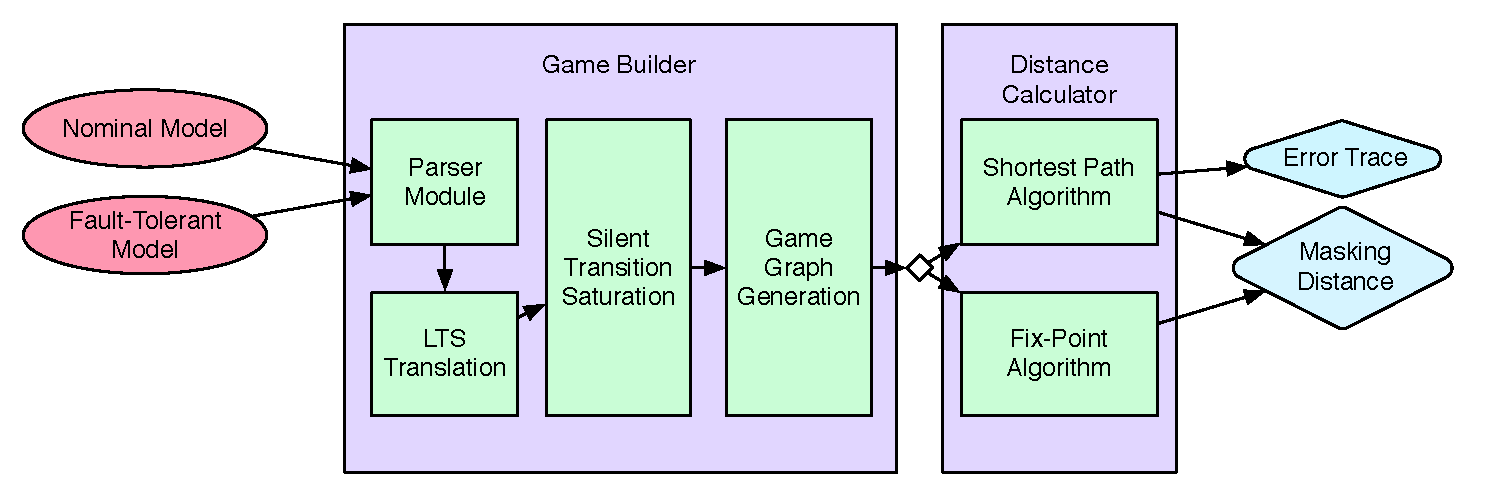
\includegraphics[scale=0.50]{Figs/architecture-eps-converted-to.pdf}
    \caption{Arquitectura de \textsf{MaskD}.}\label{fig:arch}
\end{figure}
    Discutiremos brevemente las componentes principales de la herramienta:
\begin{description}
    \item[Módulo Parser.] Realiza análisis sintáctico básico sobre los modelos de entrada y produce estructuras de datos que representan a  estas entradas. Para esto se utilizan las bibliotecas \textsf{Cup} y 
    \textsf{JFlex} para generar automáticamente el parser a partir de la gramática que describe el lenguaje de modelado.
    \item[Traducción a LTS.] Los modelos obtenidos del parser son traducidos a Sistemas de Transición Etiquetados (LTS), es decir, 
    grafos donde los vértices representan estados del programa y donde las transiciones mantienen información sobre las acciones de los modelos. 
    \item[Saturación de Transiciones Silenciosas.] Las transiciones internas/silenciosas en los LTS que representan los modelos de entrada son saturadas utilizando algoritmos estándar que provienen de teoría sobre álgebras de procesos \cite{Milner89}. Como resultado, se generan LTS saturados, estos son necesarios para verificar la relación de enmascaramiento cuando existen transiciones internas.
    \item[Generación del Grafo de Juego.] Utiliza los LTS saturados para producir un grafo de juego. Los nodos en este grafo codifican la configuración corriente del juego: 
    el próximo jugador que debe jugar, la ultima acción jugada, y referencias a los estados de los LTS de los modelos de entrada que se corresponden con la configuración actual del juego. 
    Las transiciones en este grafo corresponden a las posibles jugadas para los jugadores, es decir,  transiciones en los LTS originales.
    \item[Algoritmo de Camino mas Corto.] Si los modelos de entrada son deterministas en las etiquetas de sus acciones, el algoritmo de camino mas corto de Dial es utilizado para obtener el camino mas corto hacia el estado de error, desde el cual se calcula el valor final.
    \item[Algoritmo de Punto Fijo.] Este es el algoritmo por defecto, funciona tanto para modelos deterministas como no deterministas en las etiquetas de sus acciones, utiliza una búsqueda de estilo \textit{bottom-up breadth-first} para computar el valor del juego. 
    Este algoritmo se basa en algoritmos conocidos para resolver juegos de alcanzabilidad que utilizan conjuntos \emph{atractores} \cite{Jurd11}. 
    %This algorithm is polynomial in the game graph size.
\end{description}
Como se ha explicado mas arriba, un punto interesante sobre la herramienta es que, para sistemas deterministas en sus acciones, la distancia de enmascaramiento entre dos sistemas puede ser computada recurriendo al algoritmo de camino mas corto de Dial \cite{Dial69}, el cual tiene complejidad lineal con respecto al tamaño de los grafos utilizados para representar los sistemas.
En el caso de los sistemas no deterministas, se necesita un recorrido con punto fijo, lo cual hace que el algoritmo sea menos eficiente. Sin embargo, aun en este caso sigue siendo polinomial. 

%TODO: draw architecture and explain

%In order to measure the degree of masking fault-tolerance of a given system, 
%we start characterizing masking fault-tolerance via simulation relations between 
%two systems as defined in \cite{DemasiCMA17}. 
%The first one acting as a specification 
%of the intended behavior (es decir, nominal model) and the 
%second one as the fault-tolerant implementation (es decir, the extended model with 
%faulty behavior).
%The existence of a masking relation implies that the implementation masks the faults.
%Afterwards, we introduce a game characterization of 
%masking simulation and we enrich the resulting games 
%with quantitative objectives to define the notion of 
%\emph{masking fault-tolerance distance}, 
%where the possible values of the game belong to the interval $[0,1]$. 

\subsection{Modo de Uso}

El comando estándar para ejecutar {\MaskD} en un sistema operativo de estilo Unix es:
\\ 
\\
 \verb"./MaskD <options> <spec_path> <imp_path>"
\\
\\
En este caso la herramienta arroja como resultado la distancia de masking entre la especificación y la implementación utilizando el algoritmo por defecto (algoritmo de punto fijo).
Algunos comandos opcionales incluyen: \verb"-t: print error trace", el cual muestra por salida estándar una traza hasta el estado de error bajo estrategias óptimas; y  \verb"-s: start simulation", el cual comienza una simulación manual desde el estado inicial.  
Obtener un camino hacia el estado de error es una funcionalidad útil para encontrar defectos en las descripciones de programas, los cuales pueden fallar por razones no intencionales. A su vez la traza sirve para ver como se comportan las estrategias óptimas de los jugadores. Una traza para el ejemplo de la celda de memoria se muestra en la figura~\ref{fig:trace_mem_cell}. Los estados se muestran en el formato \verb"{spec_state, last_action_played, imp_state, player_turn}", donde \verb"spec_state" es el estado corriente del modelo nominal, \verb"last_action_played" es la última acción que se jugó (solo es relevante para estados del Verificador), \verb"imp_state" es el estado del modelo que representa a la implementación y \verb"player_turn" es el jugador cuyo turno corresponde jugar. En este caso, después de dos fallas (bits que cambian de valor sin que haya una escritura), al luego realizar una lectura, nos lleva al estado de error ya que en el modelo nominal el valor de la celda es $0$, mientras que el el modelo tolerante a fallas el valor leído en la mayoría (votación) de bits es $1$. Por otro lado, la funcionalidad de simulación permite al usuario seleccionar manualmente las acciones disponibles en cada punto del juego de enmascaramiento, lo cual también es útil para verificar que los modelos se comportan como el usuario espera.
Por defecto, \MaskD~computa la distancia de enmascaramiento para una entrada dada utilizando el algoritmo para sistemas no deterministas. 
El usuario puede utilizar la opción \verb"-det" para cambiar al algoritmo de distancia de enmascaramiento para sistemas deterministas.
\begin{figure}[t]
\centering
\begin{minipage}[t]{.47\textwidth}
\fontsize{10}{10}\selectfont\ttfamily
\begin{tabbing}
0. \{ <mr,mb0> , \# , <mr,mb0,mb1,mb2> , R \} \\ 
1. \{ <mr,mb0> , I\_m.fault1 , <mr,mb1,mb2> , V \} \\ 
2. \{ <mr,mb0> , \# , <mr,mb1,mb2> , R \} \\ 
3. \{ <mr,mb0> , I\_m.fault2 , <mb2> , V \} \\ 
4. \{ <mr,mb0> , \# , <mb2> , R \} \\ 
5. \{ <mr,mb0> , S\_m.read1 , <mb2> , V \} \\ 
6. ERR\_STATE \\ 
\end{tabbing}
\end{minipage}
\caption{Traza de Error para el ejemplo de la celda de memoria.} \label{fig:trace_mem_cell}
\end{figure}


\subsection{Evaluación Experimental} \label{sec:experimental_eval}
%\subsection{Details of the implementation}

%Las técnicas descritas en el capitulo anterior fueron implementadas en una herramienta utilizando el lenguaje \textsf{Java}, la herramienta se llama \MaskD: 
%Masking Distance Tool \cite{MaskD}. 
%\MaskD~ toma como entrada un modelo nominal y su implementación tolerante a fallas, 
%y produce como salida la distancia de masking entre ellos. 
%Los modelos son especificados utilizando el lenguaje de guardas introducido en \cite{AroraGouda93}, un lenguaje de programación simple comúnmente utilizado para describir algoritmos tolerantes a fallas.
%Mas precisamente, un programa es una colección de procesos, donde cada proceso está compuesto de una colección de acciones del estilo: $Guard \rightarrow Command$, donde $Guard$ es una condición lógica sobre el estado actual del programa y $Command$ es una colección de asignaciones básicas. Estas construcciones sintácticas se denominan acciones. El lenguaje también permite al usuario etiquetar una acción como interna (es decir, acciones $\tau$). Además, lagunas acciones pueden representar fallas en el sistema.
%La herramienta posee varias funcionalidades extra como por ejemplo mostrar trazas hacia el estado de error o iniciar una simulación desde el estado inicial.

En la Tabla~\ref{table:results} reportamos los resultados de la distancia de masking para múltiples instancias de varios casos de estudio. Estos incluyen: una Celda de Memoria Redundante (nuestro ejemplo motivador), Redundancia N-Modular (un ejemplo estándar de sistemas tolerantes a fallas \cite{ShoomanBook}), una variación del problema de los Filósofos Comensales \cite{Dijkstra71}, el problema de los Generales Bizantinos introducido por Lamport et al. \cite{LamportSP82}, una prueba de consistencia de parte del algoritmo de consenso Raft \cite{OngaroO14}, y el Protocolo de Retransmisión Acotada (un ejemplo bien conocido de un protocolo tolerante a fallas \cite{GrooteP96}). Todos los casos de estudio han sido evaluados utilizando los algoritmos para juegos deterministas y no deterministas (columnas ``Tiempo'' y ``Tiempo(Det)'', respectivamente), con la excepción de los modelos netamente no deterministas (por ejemplo, el problema de los Generales Bizantinos y el Protocolo de Retransmisión Acotada). Es de destacar que la complejidad computacional yace principalmente en la construcción explícita del grafo de juego y no del cálculo de la distancia de masking en si.

A continuación se da una interpretación de los resultados experimentales. Para el caso de una memoria redundante de $3$ bits, la distancia de masking es $0.333$. El principal motivo de esto es que el modelo con fallas, en el peor caso, solo es capaz de enmascarar $2$ fallas (en este ejemplo, una falla representa un cambio inesperado en el valor de un bit, posiblemente por una descarga) antes de fracasar al tratar de replicar el comportamiento del modelo nominal (es decir leer el valor votado por la mayoría). Por lo tanto, el resultado viene de la definición de distancia de masking y de tener en cuenta la ocurrencia de dos fallas. La situación es similar para otras instancias de este problema con mas redundancia de bits.

La Redundancia N-Modular consiste de N sistemas, los cuales desarrollan una tarea o proceso y que los resultados son procesados por un sistema de votación de mayoría para producir una única salida. 
Asumiendo un único votante perfecto, hemos evaluado este caso de estudio para diferentes cantidades de módulos.
%Note that, in this case study, the distance measuring exhibits a similar pattern to that of the 
Note que las medidas de distancia para este caso son similares al de la memoria redundante. 

\begin{table} [ht!]
\centering
\setlength{\tabcolsep}{7pt}
    \scalebox{0.85}{
  \begin{tabular}{c c c c c} \toprule
    Case de Estudio      & Redundancia & D.Masking & Tiempo & Tiempo(Det)  \\ \midrule
    \multirow{5}{*}{Celda de Memoria}          & $3$ bits & $0.333$ & $0.7$\text{s} & $0.6$\text{s}\\
                & $5$ bits & $0.25$ & $2.5$\text{s} & $1.9$\text{s}\\
                & $7$ bits & $0.2$ & $7.2$\text{s}  & $5.7$\text{s}\\
                & $9$ bits & $0.167$ & $1m.4s$ & $1$\text{m}$11$\text{s}\\
 		 	    & $11$ bits & $0.143$ & $28m27s$ & $26$\text{m}$10$\text{s}\\ \midrule
    \multirow{5}{*}{Redundancia N-Modular}           & $3$ módulos & $0.333$ & $0.6$\text{s} & $0.5$\text{s} \\
                & $5$ módulos & $0.25$ & $1.2$\text{s} & $0.7$\text{s}\\
                & $7$ módulos & $0.2$ & $5.6$\text{s}  & $3.8$\text{s}\\ 
                & $9$ módulos & $0.167$ & $2$\text{m}$55$\text{s}  & $2$\text{m}$32$\text{s}\\
 		 	    & $11$ módulos & $0.143$ & $75$\text{m}$17$\text{s}  & $72$\text{m}$48$\text{s}\\ \midrule
    \multirow{5}{*}{Filósofos Comensales}    & $2$ filósofos & $0.5$ & $0.6$\text{s} & $0.6$\text{s}\\
	            & $3$ filósofos & $0.333$ & $1.9$\text{s} & $0.9$\text{s}\\
	            & $4$ filósofos & $0.25$ & $5.9$\text{s} & $2.6$\text{s}\\ 
				& $5$ filósofos & $0.2$ & $25.3$\text{s} & $24.1$\text{s}\\ 
				& $6$ filósofos & $0.167$ & $19$\text{m}$23$\text{s} & $11$\text{m}$39$\text{s}\\ \midrule
    \multirow{3}{*}{Generales Bizantinos}    
                & $3$ generales & $0.5$ & $0.9$\text{s} & $-$ \\
            	& $4$ generales & $0.333$ & $17.1$\text{s} & $-$\\ 
            	& $5$ generales & $0.333$ & $429$\text{m}$54$\text{s} & $-$\\ \midrule
    \multirow{3}{*}{Raft LRCC (5)}        & $1$ seguidor & $0$ & $0.7$\text{s} & $0.8$\text{s}\\
            & $2$ seguidores & $0$ & $5.6$\text{s} & $3.6$\text{s} \\ 
            & $3$ seguidores & $0$ & $49$\text{m}$50$\text{s} & $37$\text{m}$53$\text{s} \\ \midrule
    \multirow{5}{*}{BRP(1)}       	& $1$ retransm. & $0.333$ & $0.7$\text{s} & $-$\\ 
 						& $5$ retransm. & $0.143$ & $0.8$\text{s}  & $-$\\ 
 						& $10$ retransm. & $0.083$ & $1.3$\text{s}  & $-$\\ 
 						& $20$ retransm. & $0.045$ & $3.9$\text{s}  & $-$\\ 
 						& $40$ retransm. & $0.024$ & $4.8$\text{s} & $-$ \\ \midrule
	\multirow{5}{*}{BRP(5)}       	& $1$ retransm. & $0.333$ & $4.2$\text{s} & $-$\\
					& $5$ retransm. & $0.143$ & $4.8$\text{s}  & $-$\\ 
					& $10$ retransm. & $0.083$ & $6.1$\text{s}  & $-$\\ 
					& $20$ retransm. & $0.045$ & $8.7$\text{s}  & $-$\\ 
					& $40$ retransm. & $0.024$ & $18.6$\text{s} & $-$ \\ \midrule
	\multirow{5}{*}{BRP(10)}       	& $1$ retransm. & $0.333$ & $4.7$\text{s} & $-$\\ 
					& $5$ retransm. & $0.143$ & $6.4$\text{s} & $-$ \\ 
					& $10$ retransm. & $0.083$ & $10.1$\text{s} & $-$ \\
					& $20$ retransm. & $0.045$ & $20.5$\text{s} & $-$ \\ 
					& $40$ retransm. & $0.024$ & $1$\text{m}$9$\text{s} & $-$ \\ \bottomrule
  \end{tabular}}
\vspace{0.2cm}
\caption{Resultados de la distancia de masking para los casos de estudio.}
\vspace{-0.8cm}
\label{table:results}
\end{table} 

Para el problema de los filósofos comensales, adaptamos la implementación par/impar en la cuál algunos filósofos obtienen primero el tenedor derecho y otros obtienen primero el izquierdo. Específicamente tenemos $n-1$ filósofos \emph{impares} que obtienen el tenedor derecho primero, y $1$ filósofo \emph{impar} que obtiene primero el izquierdo. En este caso, consideramos que ocurre una falla cuando un filósofo impar actúa como uno par, esto se puede entender como una falla bizantina. Para dos filósofos la distancia de masking es $0{.}5$ ya que basta con una falla para alcanzar un estado de deadlock. Mientras mas filósofos la distancia de masking se vuelve mas pequeña. 
%We have evaluated this problem on four instances with $2, 3, 4,$ and $5$ philosophers, respectively.

%\hrmkPRD{Explicar el de los Generales Bizantinos!!}
Otro ejemplo interesante de un sistema tolerante a fallas es el problema de los generales bizantinos, introducido originalmente por Lamport et al. \cite{LamportSP82}. Este es un problema de consenso, donde hay un general comandante con $n-1$ tenientes. La comunicación entre el general y sus tenientes ocurre a través de mensajeros. El general puede decidir entre atacar la ciudad enemiga o retirarse; luego, manda la orden a sus tenientes. Algunos de estos pueden ser traidores. 
Asumimos que los mensajes son entregados sin problemas y que todos los tenientes pueden comunicarse entre si de forma directa. Bajo este escenario ellos pueden reconocer quien mandó un mensaje. Las fallas pueden convertir a un teniente leal en un traidor (fallas bizantinas). En consecuencia, los traidores pueden mandar mensajes falsos o incluso omitir mandar los mensajes que recibieron a otros tenientes. Los tenientes leales deben acordar atacar o retirarse después de $m + 1$ rondas de comunicación, donde $m$ es el máximo número de traidores. Aquí consideramos el caso de $m=1$.  

%The algorithm can ensure correct operation only if fewer than one third of the lieutenants are traitors.

Raft \cite{OngaroO14} es un algoritmo de consenso que se ha vuelto popular en años recientes. En Raft, un líder es elegido de un conjunto de servidores disponibles, una vez electo, el líder recibe peticiones de clientes y las reenvía a sus seguidores (los demás servidores), así pueden replicar la información nueva en sus estados respectivos. Cada servidor mantiene un historial de las entradas recibidas. Un seguidor puede rechazar una entrada si existe alguna inconsistencia entre su historial y el historial del líder, esto se considera una falla en nuestro contexto. Cuando esto ocurre, el líder intenta nuevamente con la entrada anterior de su historial, esto se repite hasta que sea congruente con la entrada mas reciente del seguidor en conflicto. Aquí modelamos solo una de las etapas del algoritmo Raft, la etapa de Replicación de Historial. Específicamente, adaptamos el control de consistencia que realiza el protocolo para asegurar consistencia entre los historiales de los seguidores y el historial del líder. Computamos la distancia de masking para este modelo con $1$, $2$ y $3$ seguidores, y considerando un historial del líder de $5$ entradas. Notemos que esta distancia es siempre $0$. Intuitivamente, esto ocurre porque, a pesar de que puede haber rechazos, eventualmente todos los historiales van a estar de acuerdo (en el peor caso, el protocolo va a descartar todas las entradas de los seguidores hasta alcanzar un historial vacío, y luego copiarán todas las entradas del historial del líder en sus respectivos historiales). 

El Protocolo de Retransmisión Acotada o Bounded Retransmission Protocol (BRP) es un caso de estudio sobre verificación de software conocido en el ámbito industrial. Mientras los demás casos de estudio han sido tratados como "ejemplos de juguete" y analizados con $\DeltaMask$, el BRP fue modelado de forma mas cercana a una implementación siguiendo~\cite{GrooteP96}, considerando diferentes componentes (emisor, receptor, y canales). Para analizar tal modelo utilizamos la distancia de masking débil $\DeltaMask^W$.
Hemos calculado la distancia de masking para el protocolo con $1$, $5$ y $10$ trozos de mensaje a enviar, denotados BRP(1), BRP(5) y BRP(10), respectivamente. 

Podemos observar que los valores de la distancia no son afectados por la cantidad de trozos a enviar por el protocolo. Esto es de esperar, debido a que la distancia de masking depende de la redundancia agregada para enmascarar fallas, en este caso, depende de la cantidad de retransmisiones permitidas.

Los experimentos fueron realizados en una MacBook Air con un procesador Intel Core i5 de 1.3 GHz y una memoria RAM de 4GB. El código fuente y los archivos ejecutables de la herramienta así como los casos de estudio para reproducir los resultados se encuentran disponibles en un repositorio Github \cite{MaskD}.





\section{Trabajo Relacionado} \label{sec:related_work_mask}

En los últimos años, se ha incrementado el interés en generalizaciones cuantitativas de la noción booleana de correctitud y sus interrogantes correspondientes en verificación cuantitativa \cite{BokerCHK14,CernyHR12,Henzinger10,Henzinger13}.
El framework descrito en \cite{CernyHR12} es el trabajo mas cercanamente relacionado a nuestro enfoque. 
Los autores generalizan la noción tradicional de relación de simulación a tres versiones diferentes de distancia de simulación: \emph{correctitud}, \emph{cobertura}, y \emph{robustez}.
Estas están definidas utilizando juegos cuantitativos con objetivos \emph{discounted-sum} 
y \emph{mean-payoff}, dos funciones de costo bien conocidas.
Similarmente a ese trabajo, también consideramos distancias entre sistemas puramente discretos (no probabilistas y sin tiempo.

Las distancias de correctitud y cobertura se concentran en la parte nominal de los sistemas, y por lo tanto las fallas no cumplen un rol en estas distancias. Por otro lado, la distancia de robustez mide cuantos errores inesperados pueden ocurrir en la implementación de tal forma que el comportamiento resultante es tolerado por la especificación. Entonces, esta distancia puede ser utilizada para analizar la resiliencia de la implementación. Notemos que, la distancia de robustez solo puede ser aplicada a implementaciones correctas, es decir, implementaciones que preserven el comportamiento de la especificación pero tal vez no cubre todo su comportamiento. 
 Como ha sido notado en~\cite{CernyHR12}, la bisimilitud a veces implica una distancia de $1$. En este sentido, un grado mayor de robustez (como está definido en~\cite{CernyHR12}) se logra al recortar puntos críticos de la especificación. Además, los errores considerados en ese trabajo son transiciones que imitan a las originales pero con diferentes etiquetas. En contraste con esto, nuestro enfoque considera que las fallas son inyectadas en la implementación tolerante a fallas, donde sus comportamientos no son restringidos por el sistema nominal. Esto sigue la idea de la extensión de modelos en tolerancia a fallas donde se agrega comportamiento defectuoso al sistema nominal. Además, notemos que cuando no ocurren fallas, la distancia de masking entre la especificación y la implementación es $0$ cuando son bisimilares, y es  $1$ en caso contrario.
Es útil destacar que la distancia de robustez de~\cite{CernyHR12} no es reflexiva. Creemos que todas estas definiciones de distancia entre sistemas capturan diferentes nociones útiles para el desarrollo de software, y pueden ser utilizadas en conjunto, de forma complementaria, para obtener una evaluación profunda de implementaciones tolerantes a fallas.








